\documentclass{tufte-handout}

%\geometry{showframe}% for debugging purposes -- displays the margins

\usepackage{amsmath}

\usepackage{ulem}
% Set up the images/graphics package
\usepackage{graphicx}
\setkeys{Gin}{width=\linewidth,totalheight=\textheight,keepaspectratio}
\graphicspath{{graphics/}}

\title{Hierarchical approach for determining distribution of parameters consistent with experiments measuring transport of water in PMMA}
\author[]{}
%\date{}  % if the \date{} command is left out, the current date will be used

% The following package makes prettier tables.  We're all about the bling!
\usepackage{booktabs}

% The units package provides nice, non-stacked fractions and better spacing
% for units.
\usepackage{units}

% The fancyvrb package lets us customize the formatting of verbatim
% environments.  We use a slightly smaller font.
\usepackage{fancyvrb}
\fvset{fontsize=\normalsize}

% Small sections of multiple columns
\usepackage{multicol}

% Provides paragraphs of dummy text
\usepackage{lipsum}

% These commands are used to pretty-print LaTeX commands
\newcommand{\doccmd}[1]{\texttt{\textbackslash#1}}% command name -- adds backslash automatically
\newcommand{\docopt}[1]{\ensuremath{\langle}\textrm{\textit{#1}}\ensuremath{\rangle}}% optional command argument
\newcommand{\docarg}[1]{\textrm{\textit{#1}}}% (required) command argument
\newenvironment{docspec}{\begin{quote}\noindent}{\end{quote}}% command specification environment
\newcommand{\docenv}[1]{\textsf{#1}}% environment name
\newcommand{\docpkg}[1]{\texttt{#1}}% package name
\newcommand{\doccls}[1]{\texttt{#1}}% document class name
\newcommand{\docclsopt}[1]{\texttt{#1}}% document class option name

\begin{document}

\maketitle% this prints the handout title, author, and date

%\begin{abstract}
%\noindent This document describes the Tufte handout \LaTeX\ document style.
%It also provides examples and comments on the style's use.  Only a brief
%overview is presented here; for a complete reference, see the sample book.
%\end{abstract}

%\printclassoptions


\section{Experimental Data}
The available experiments measure the `water vapor transport rate', or the flux
of water through a nominally 1D geometry of the test sample. The experiment
begins by establishing a `dry' sample by flowing dry air through the
measurement chambers, then switches to a fixed temperature and relative
humidity on one side of the sample. The other side of the sample is maintained
at $\sim 0\%$ relative humidity and the flux of water out of the sample is
measured. An analytic solution is available. The model is:
\begin{marginfigure}%
    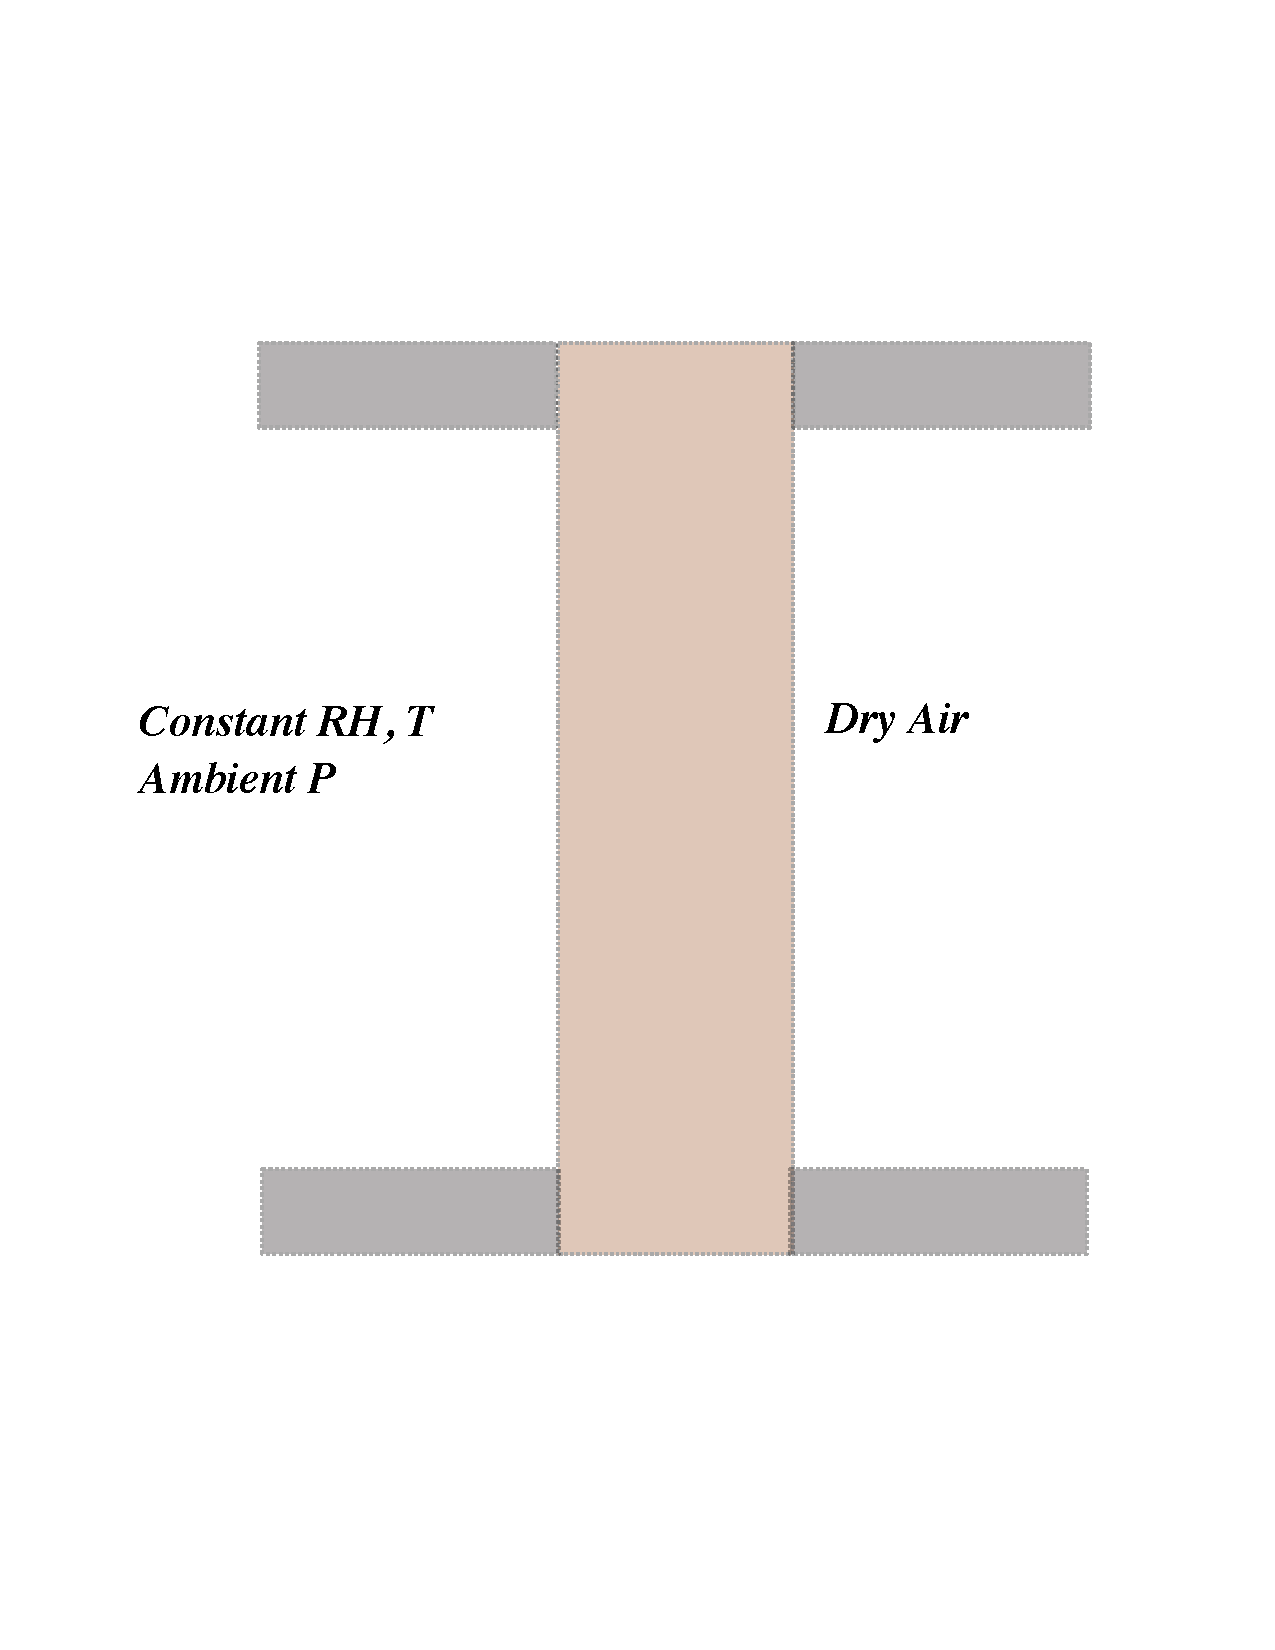
\includegraphics[width=1.0\linewidth]{WVTR.pdf}
    \caption{
    Measurements taken with MOCON Permatran; output of experimental measurement
is time trace of water vapor transport rate }
    \label{fig:marginfig}
\end{marginfigure}

\begin{equation} \frac{\partial C}{\partial t} =
    \frac{\partial}{\partial x} D \frac{\partial C}{\partial x}
\end{equation}

\begin{itemize}
  \item Dirichlet boundary conditions:
      \begin{itemize}
          \item $C=k_Da$ at $x=0$
          \item $C=0$ at $x=L$
          \item $a$ is activity; $a = (RH)\left.\frac{P_{\mathrm{sat}}}{P_{\mathrm{a}}}\right|_{T_\mathrm{amb}}$
        \end{itemize}
   \item Closed form solution 
       \begin{equation}
           \mathrm{WVTR} = \frac{DKa}{L}\sum_{n=0}^{\infty} 2(-1)^ne^{-Dn^2\pi^2(t-t_0)/l^2}
       \end{equation}
\end{itemize}

Both parameters ($D,K$) have an exponential temperature dependence.
\begin{gather}
        D = D_0 e^{D_1/T}\\
        K = K_0 e^{K_1/T}
\end{gather}
Four experiments are available at various temperatures. 

\section{Normalizing experimental data}
\newthought{The experiments should have the same importance}, or at least they
should not have different influence simply due to the number of data points
extracted. Scaling the probabilities by raising the probability for a each
experiment to the $\frac{1}{N}^{th}$ power, where $N$ is the number of sample
points is the current approach to address this. That is, for the lnlikihood for
$M$ experiments with $N_m$ datapoints
\begin{equation}
    F_D = \sum_{m=1}^{M} \left[ -0.5\frac{1}{N_m} \sum_{n=1}^{N_m} (f_{m,n}^{\mathrm{model}} - f_{m,n}^{\mathrm{measured}})^2 \frac{1}{\sigma_{m,n}^2} \right]
    \label{eq:FD}
\end{equation}


\section{ToDo List}
\newthought{The premise} is that model for experiment \#2 is more expensive
than \#1, and we are conducting an experiment to see if we can reduce the
number of evaluations of the model for \#2 by using a hierarchical approach.
\begin{enumerate}
    \item Run emcee sampler on $p(\phi|Z_1,Z_2)$, that is, using all of the
        experimental data for a `large' number of samples. This will serve as
        `ground truth', with large being $\sim 4(10^6)$ per walker (8 walkers).
        Initial walker positions in a small ball around the MLE.
    \item Run emcee sampler on experiment \#1 only, to determine $p(\phi|Z_1)$.
        Do this several times in sequence, each time drawing the initial walker
        positions from the prior. Take `many' (e.g., 4M) samples. For the first
        attempt, use a very broad prior to draw samples for initial walker
        position.\footnote{This is a bit contrived, but the supposition is that
        we are not able to determine the MLE solution. So we are using sampling
    to reduce the space with each successive run and are putting the walkers in
a better position.}
    \item Sample the final posterior from experiment \#1 to get initial walker
        positions for the next step. Also bin the posterior samples to obtain a
        representation of the distribution $\mu_{H}^1(D_0,D_1,K_0,K_1|Z_1)$
        that can be evaluated at an arbitrary $(D_0,D_1,K_0,K_1)$.
    \item Run the emcee sampler on $p(\phi|Z_1,Z_2)$, but this time use initial
        walker positions obtained through consideration of Experiment \#1, and
        use $\mu_H^1$ as the prior\footnote{Using the prior facilitates an
        optimization where we don't bother evaluating the sample if the prior
    is $< p_{min}$}. Compare the posterior to the baseline
        posterior obtained in the first step.  Take fewer (e.g., 100k) samples. 
    \item Run the emcee sampler on $p(\phi|Z_2)$, using $\mu_H$ as a prior.
        Compare the posterior to the baseline posterior from the first step.
    \item Redo the first step, but use only the number of samples corresponding
        to the number of function evaluations for Expt. \#2 in the hierarchical
        approach.
    \item Alternatively, everywhere emcee sampler is used, attempt GD
        optimization starting from the walker positions, and if successful use
        IS in place of emcee sampler. 
\end{enumerate}

\section{Progress}
\newthought{The baseline sampling}, starting the walkers from a ball
around the MLE (from the `2 step' procedure), and taking 4M samples
for each of 8 walkers produces:
\begin{figure}
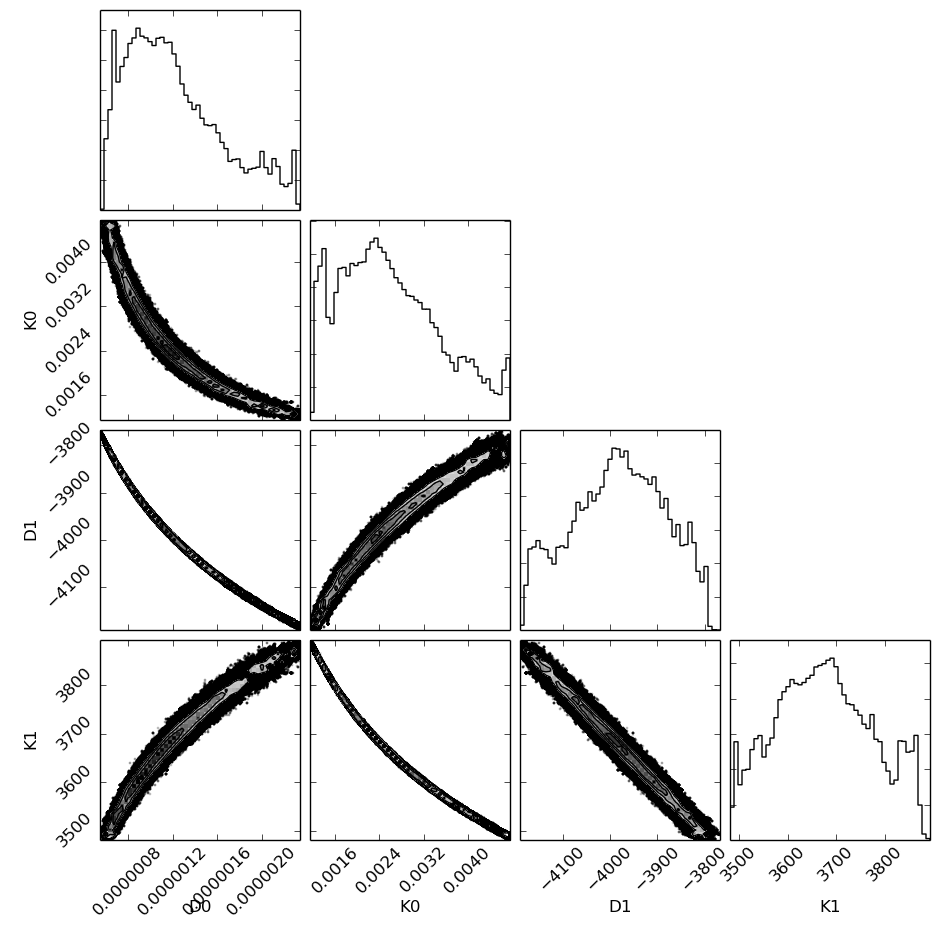
\includegraphics[width=\columnwidth]{figs/step_1_4M_2exp.png}
  \caption{Baseline starting walkers near the MLE.}
  \label{fig:baseline}
  \setfloatalignment{b}
\end{figure}

\newthought{Without annealing} the hierarchical process fails to
provide anything useful; indeed, when the walkers are placed uniformly
throughout the valid bounds over which the prior has uniform
probability they become `stuck'. However, with suitable annealing, it
seems possible to produce a posterior that is evolving towards
something sensible\sout{---although, it seems, inconsistent with the
baseline}\footnote{Now that I am doing this for a consistent set of bounds / experiments it doesn't look too bad}. In Figure \ref{fig:annealing}, the walkers were initially
placed uniformly across the valid region for the initial 'broad'
prior. For subsequent experiment the walker positions were chosen
randomly from the samples from the previous experiment. 50k samples per walker were taken.
\begin{figure}
$\begin{array}{c c}
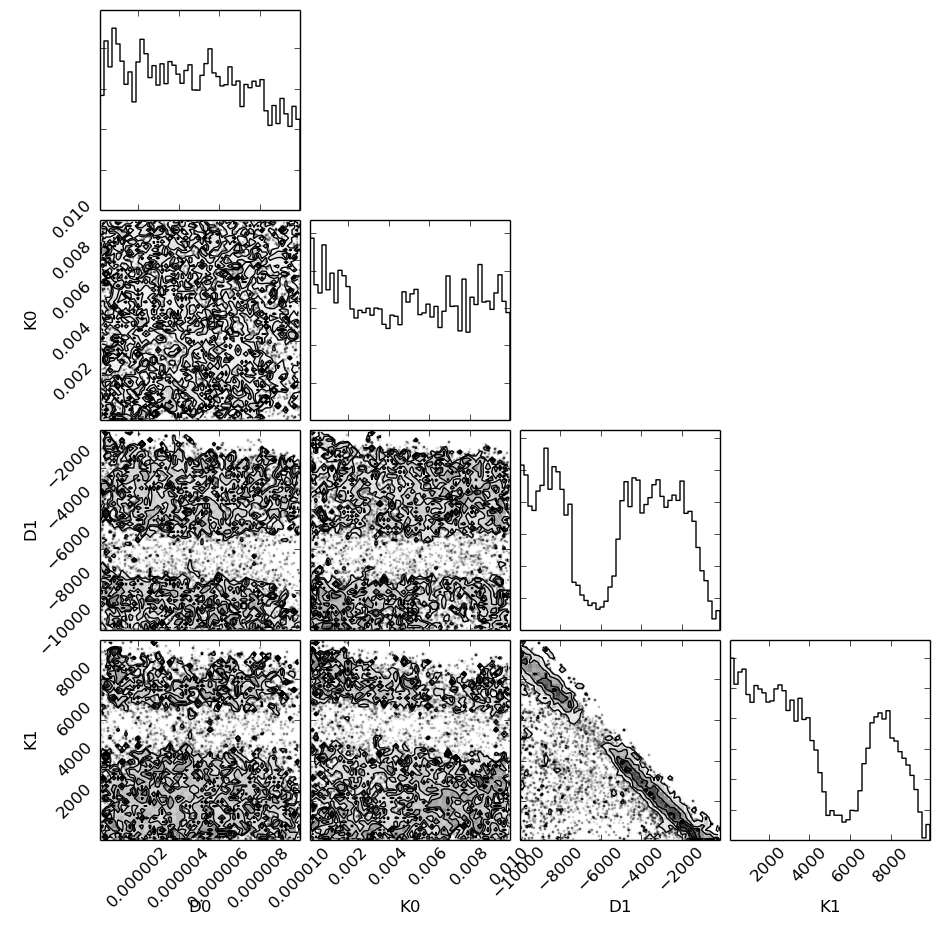
\includegraphics[width=0.48\columnwidth]{figs/50k_annealing_noclustering/triangle_seq_prior_0.png}
& 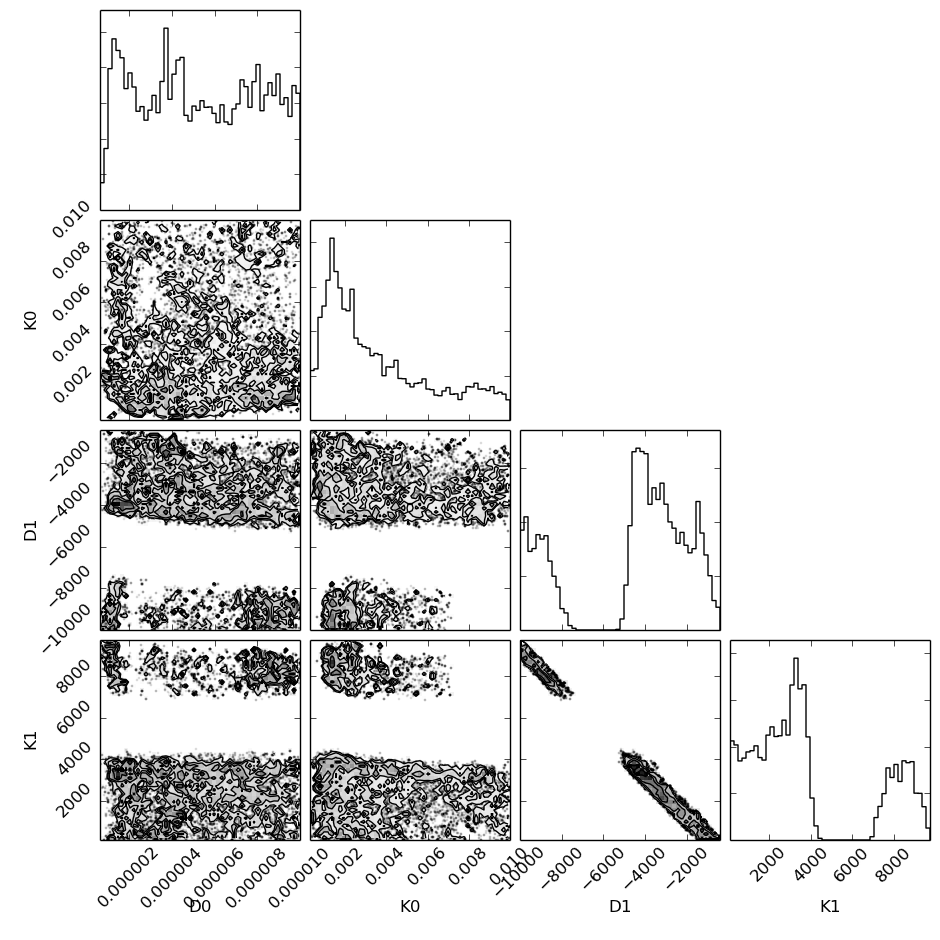
\includegraphics[width=0.48\columnwidth]{figs/50k_annealing_noclustering/triangle_seq_prior_1.png}
\\
n=0 & n=1 \\
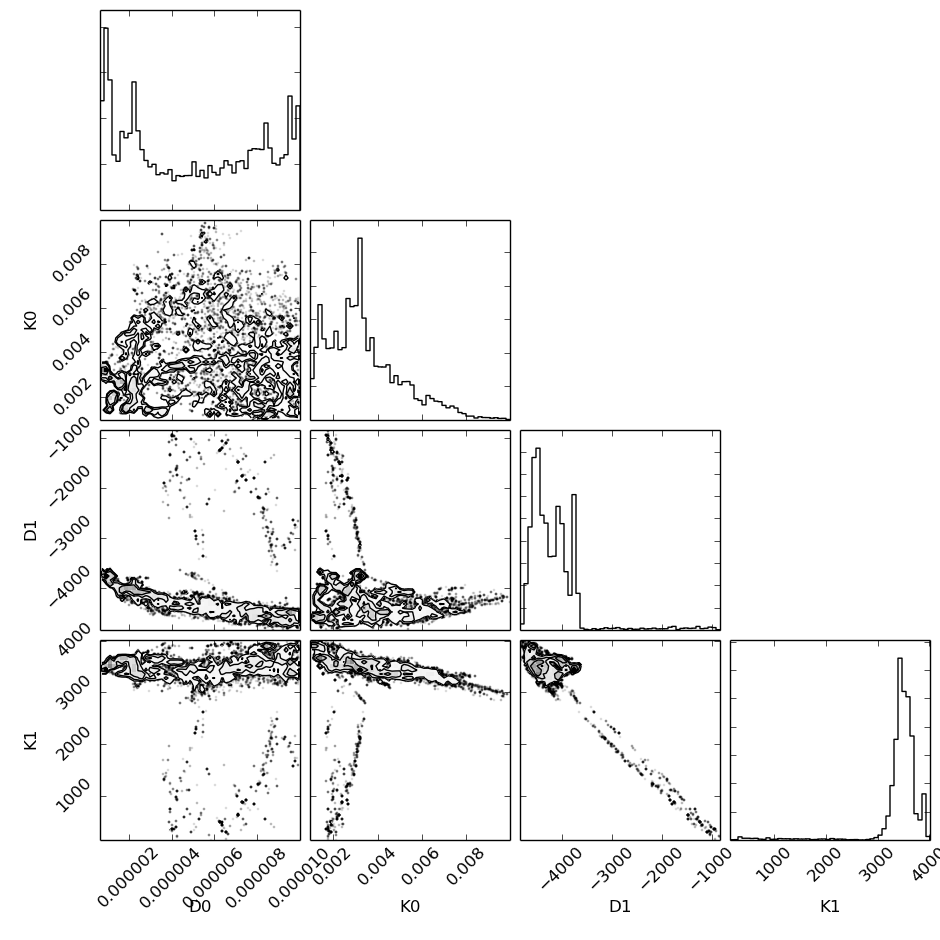
\includegraphics[width=0.48\columnwidth]{figs/50k_annealing_noclustering/triangle_seq_prior_2.png}
& 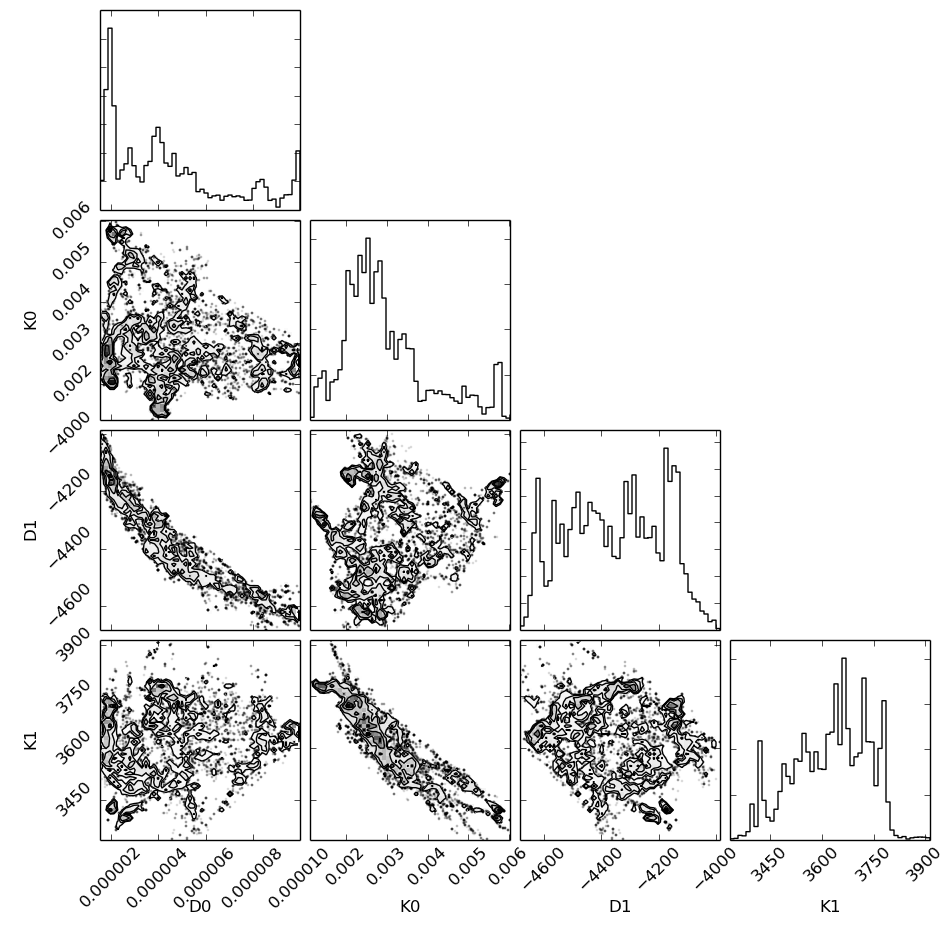
\includegraphics[width=0.48\columnwidth]{figs/50k_annealing_noclustering/triangle_seq_prior_3.png}
\\
n = 2 & n=3 \\
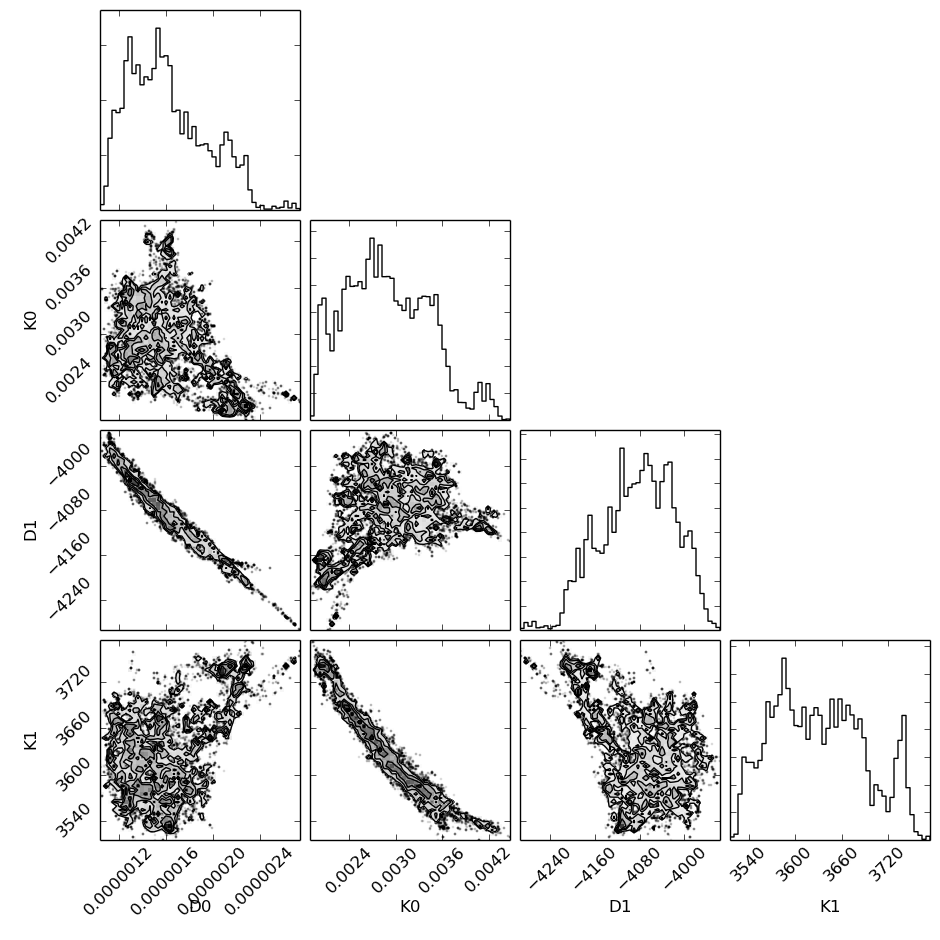
\includegraphics[width=0.48\columnwidth]{figs/50k_annealing_noclustering/triangle_seq_prior_4.png}
& 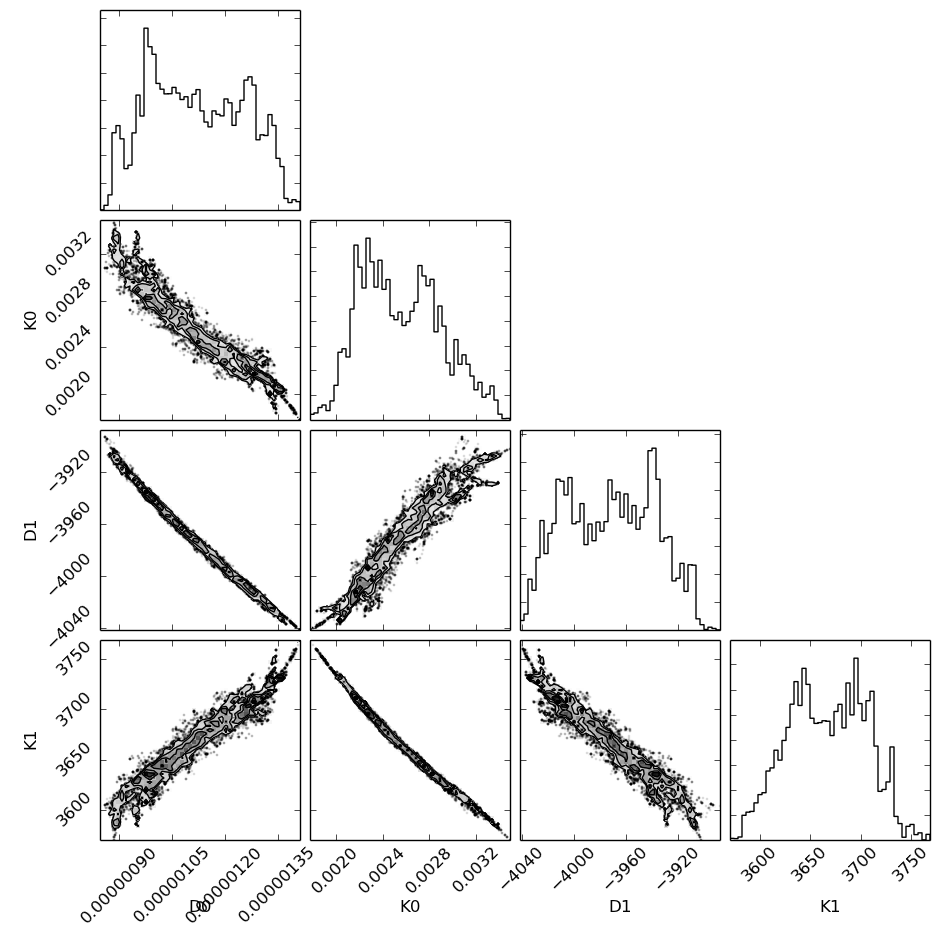
\includegraphics[width=0.48\columnwidth]{figs/50k_annealing_noclustering/triangle_seq_prior_5.png} \\
n = 4 & n=5 \\
\end{array}$
  \caption{Baseline starting walkers uniformly across bounds, using
    annealing process where $\sigma = \sigma_0*(1+98)e^{-(5/4) n}$,
    where $n$ is the index of the pseudo-experiment. $n=4$ was
    experiment \#1 with $\sigma=\sigma_0$, and $n=5$ was both
    experiments \#1 and \#2.}
  \label{fig:annealing}
  \setfloatalignment{b}
\end{figure}

\sout{Sadly, this doesn't appear to be robust;}\footnote{Not sure
about this now, redoing the runs right now} I repeated the run with a larger
sample count ($10^6$/walker), but otherwise the same annealing schedule. Results are shown 
in Figure~\ref{fig:annealing2}

%and the walkers managed to find the `wrong' probability island. In an
%attempt to fix this, I choose $50(10^3)$ samples randomly from the
%previous posterior, sorted these
%by likelyhood, and chose 8 at random from the 99$^{th}$ percentile to
%initialize the worker positions --- this is what is shown in Figure~\ref{fig:annealing2}.
\begin{figure}[h!]
$\begin{array}{c c}
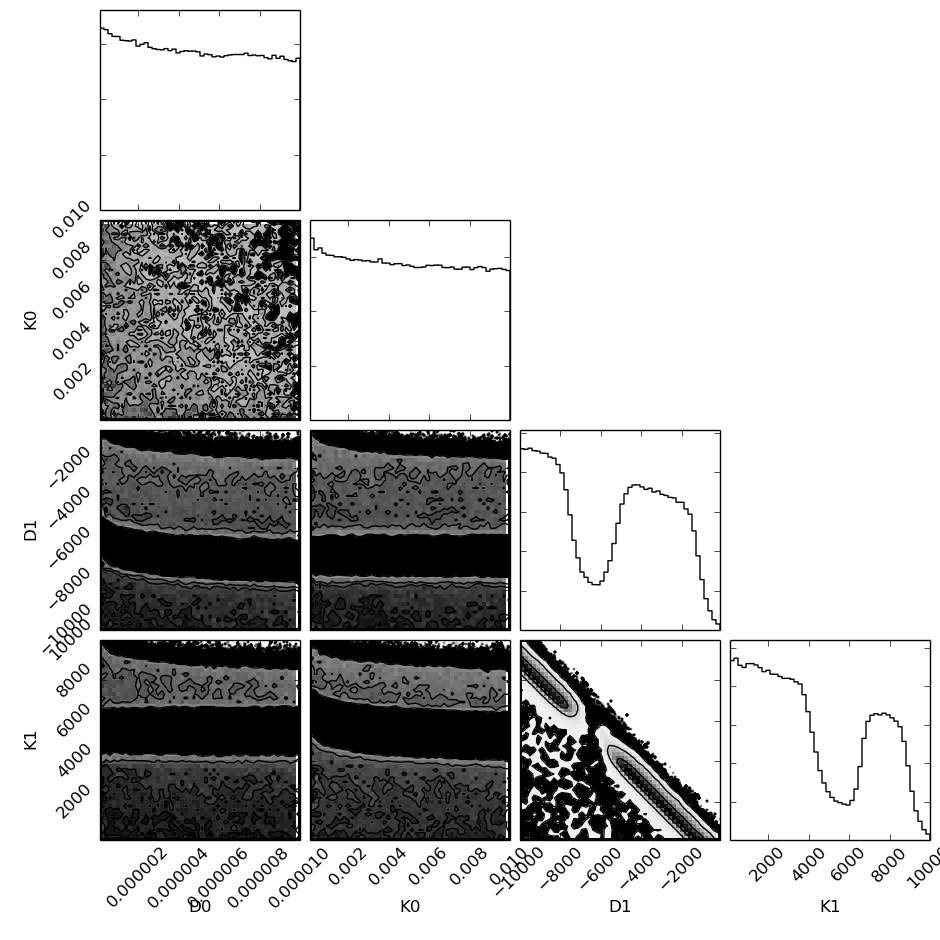
\includegraphics[width=0.48\columnwidth]{figs/1M_annealing_norm/triangle_seq_prior_0.png}
& 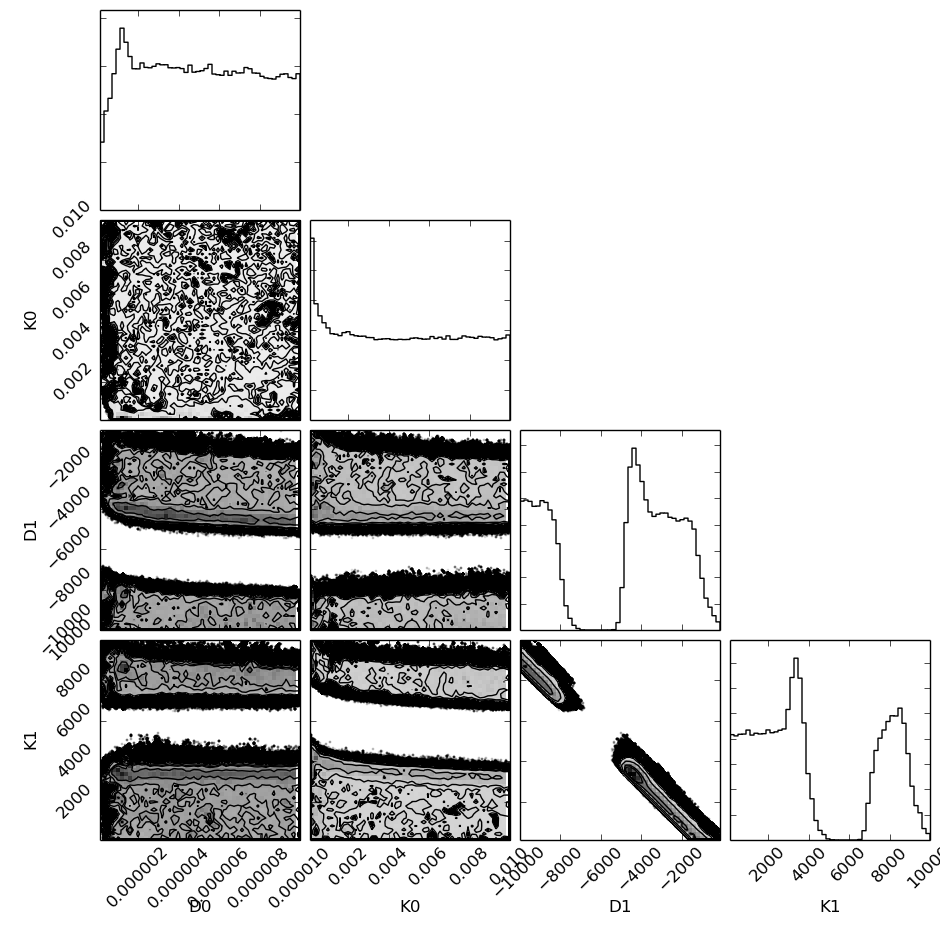
\includegraphics[width=0.48\columnwidth]{figs/1M_annealing_norm/triangle_seq_prior_1.png}
\\
n=0 & n=1 \\
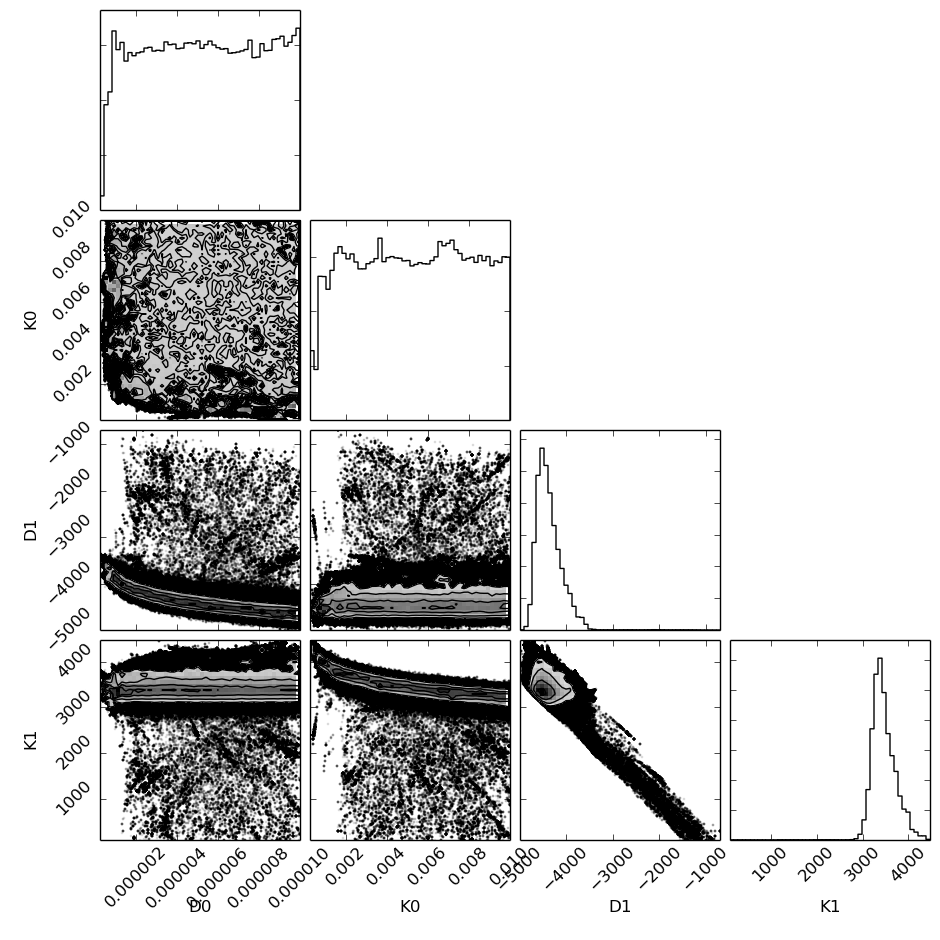
\includegraphics[width=0.48\columnwidth]{figs/1M_annealing_norm/triangle_seq_prior_2.png}
& 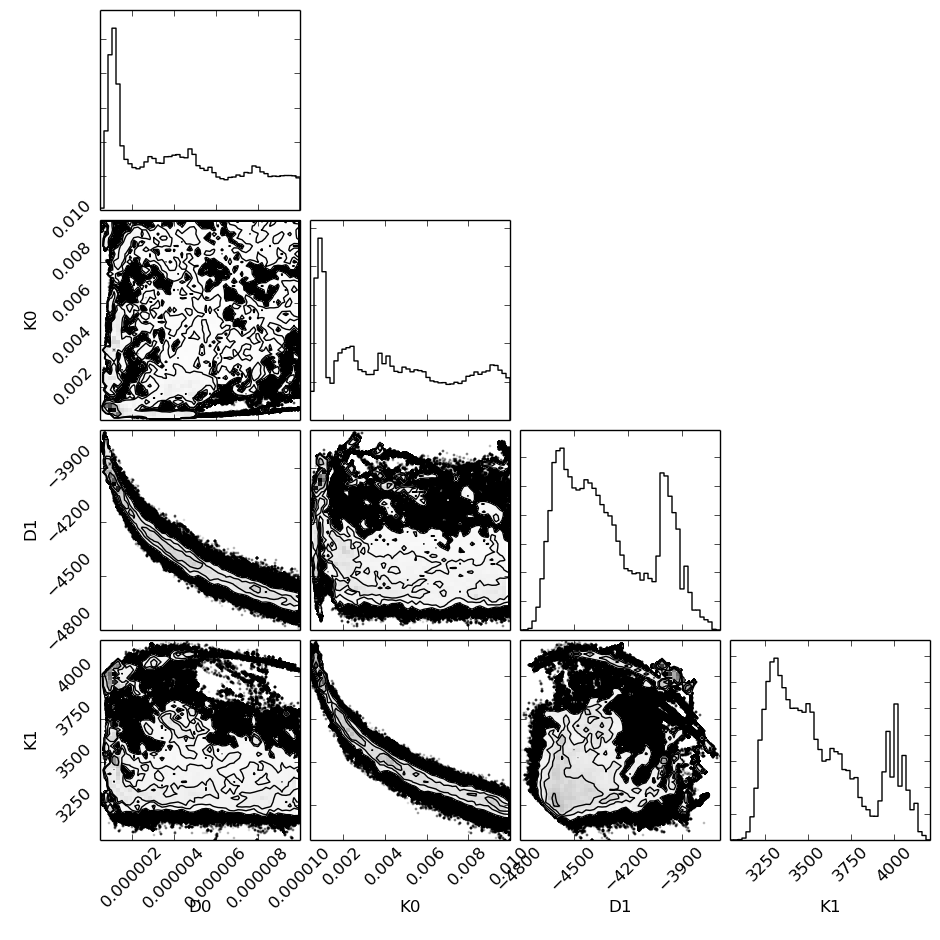
\includegraphics[width=0.48\columnwidth]{figs/1M_annealing_norm/triangle_seq_prior_3.png}
\\
n = 2 & n=3 \\
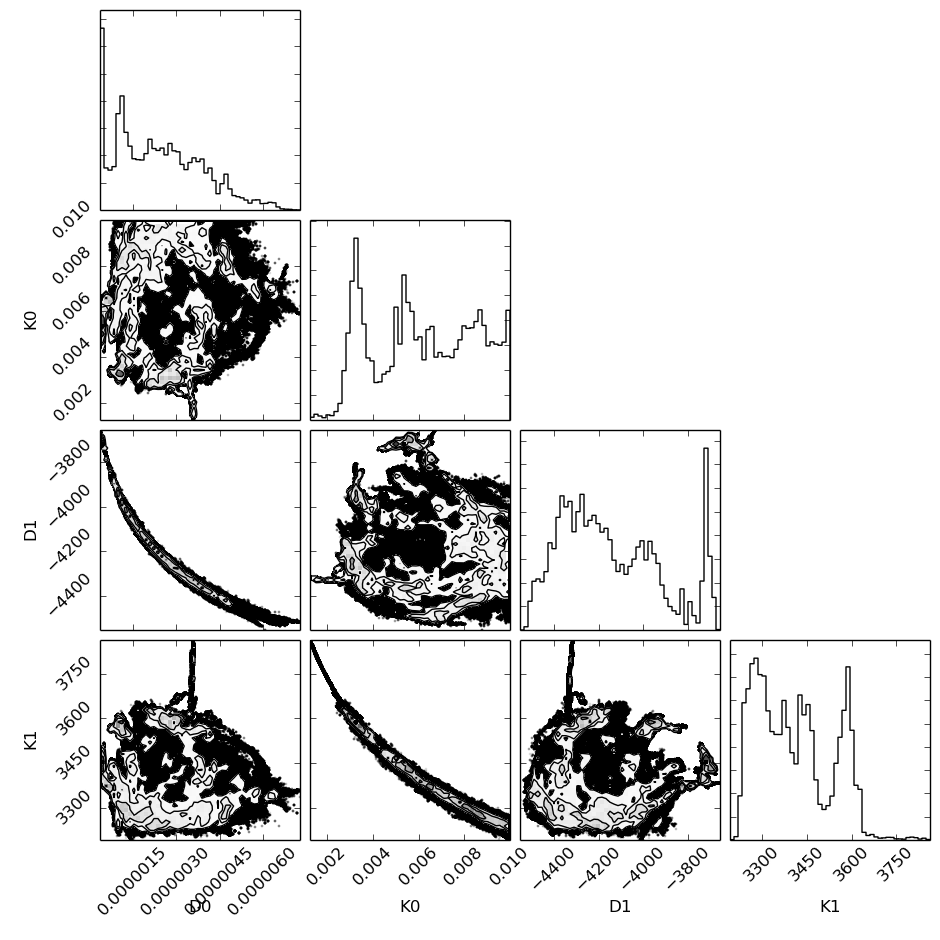
\includegraphics[width=0.48\columnwidth]{figs/1M_annealing_norm/triangle_seq_prior_4.png}
& 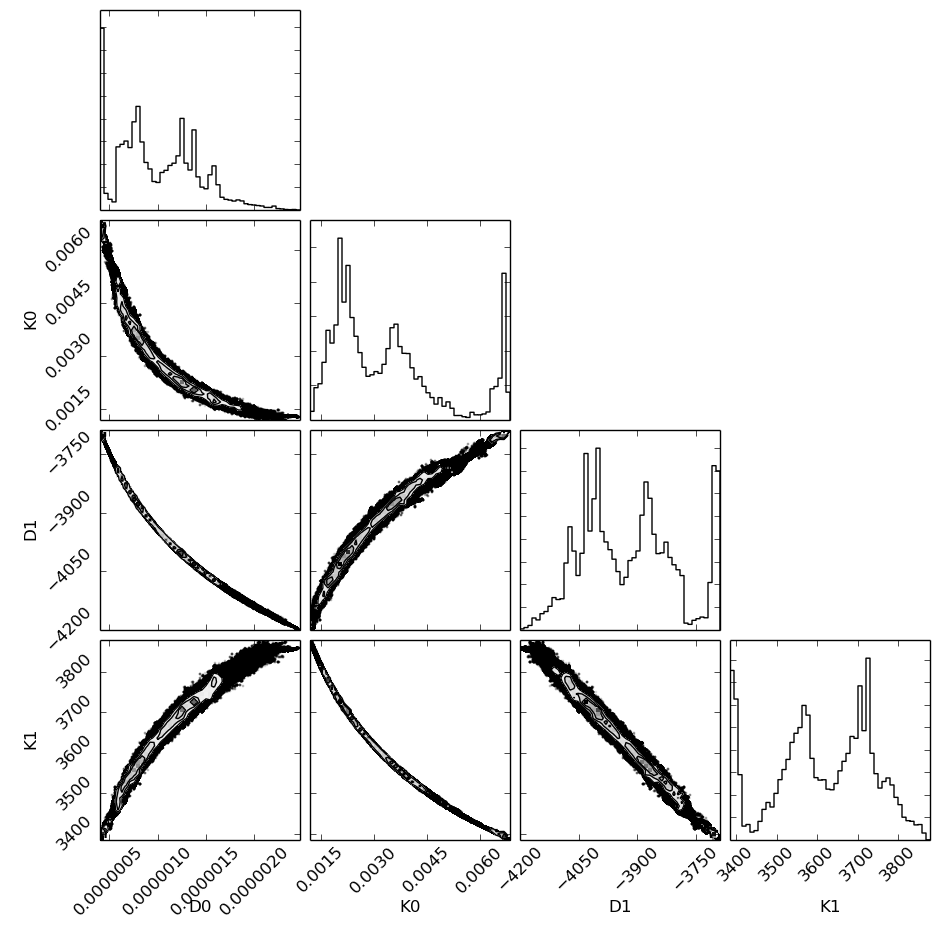
\includegraphics[width=0.48\columnwidth]{figs/1M_annealing_norm/triangle_seq_prior_5.png} \\
n = 4 & n=5 \\
\end{array}$
  \caption{Starting walkers uniformly across bounds, using
    annealing process where $\sigma = \sigma_0*(1+98)e^{-(5/4) n}$,
    where $n$ is the index of the pseudo-experiment. $n=4$ was
    experiment \#1 with $\sigma=\sigma_0$, and $n=5$ was both
experiments \#1 and \#2. $10^6$ samples per walker. This is using normalized likelihood ($1/N_m$).}
  \label{fig:annealing2}
  \setfloatalignment{b}
\end{figure}

\newthought{Since Matti doesn't like normalizing the likelihood}, I repeated
the exercise without the $1/N_m$ factor from Eqn.~\ref{eq:FD}. Then the
baseline looks like Figure~\ref{fig:baseline_nonorm}. The darn thing looks Gaussian!
\begin{figure}
    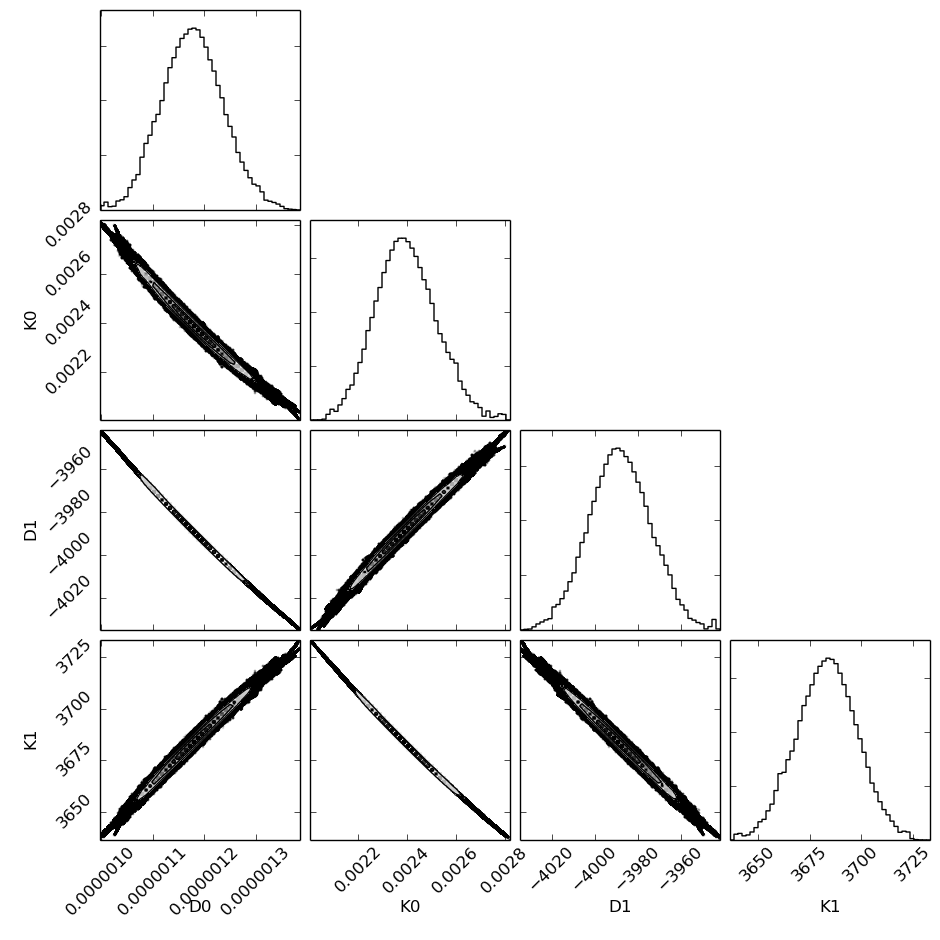
\includegraphics[width=\columnwidth]{figs/baseline_no_norm/triangle_global.png}
    \caption{Baseline starting walkers near the MLE, no $1/N_m$ factor, 4M samples per walker (8 walkers).}
  \label{fig:baseline_nonorm}
  \setfloatalignment{b}
\end{figure}

Then, the experiment with the hierarchical approach is shown in Fig.~\ref{fig:annealing_nonorm}. 
\begin{figure}[h!]
$\begin{array}{c c}
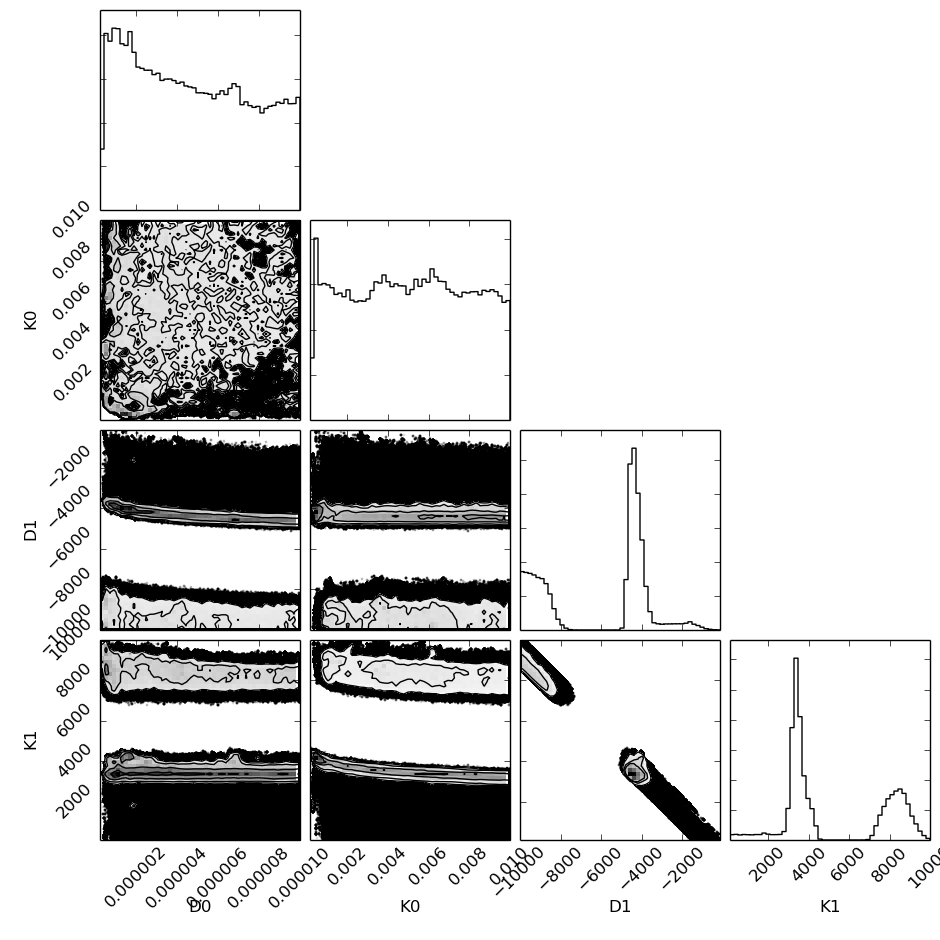
\includegraphics[width=0.48\columnwidth]{figs/1M_annealing_no_norm/triangle_seq_prior_0.png}
& 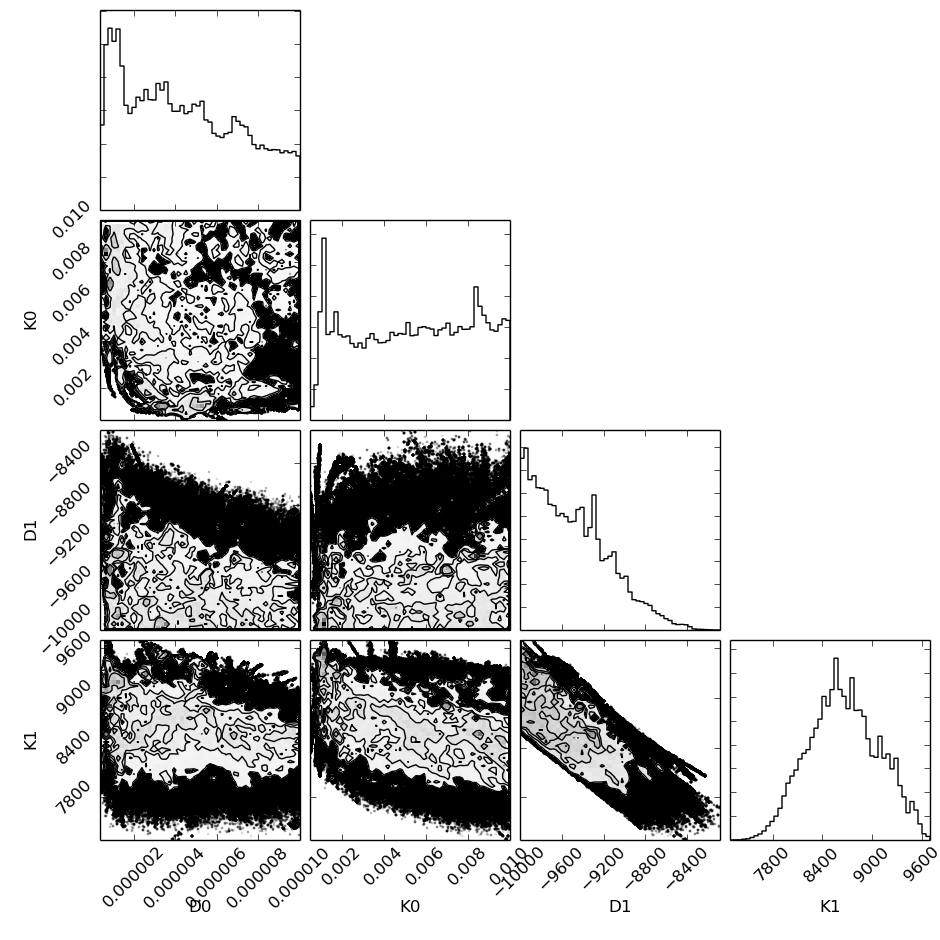
\includegraphics[width=0.48\columnwidth]{figs/1M_annealing_no_norm/triangle_seq_prior_1.png}
\\
n=0 & n=1 \\
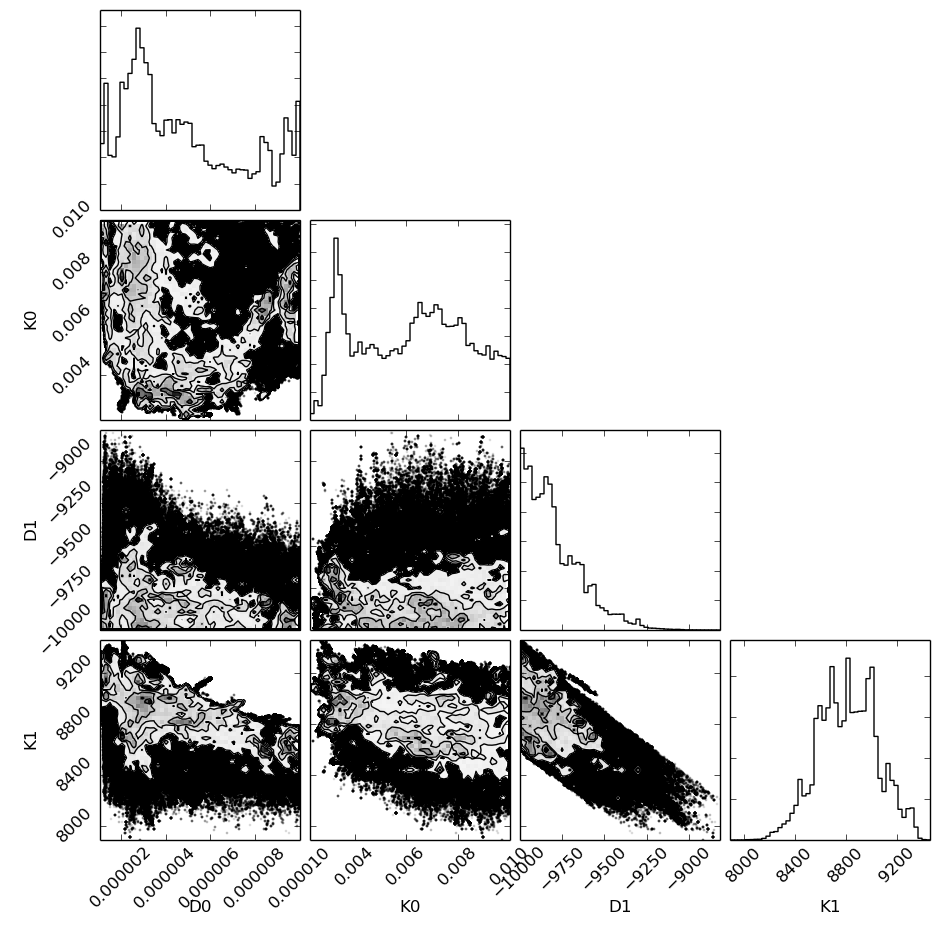
\includegraphics[width=0.48\columnwidth]{figs/1M_annealing_no_norm/triangle_seq_prior_2.png}
& 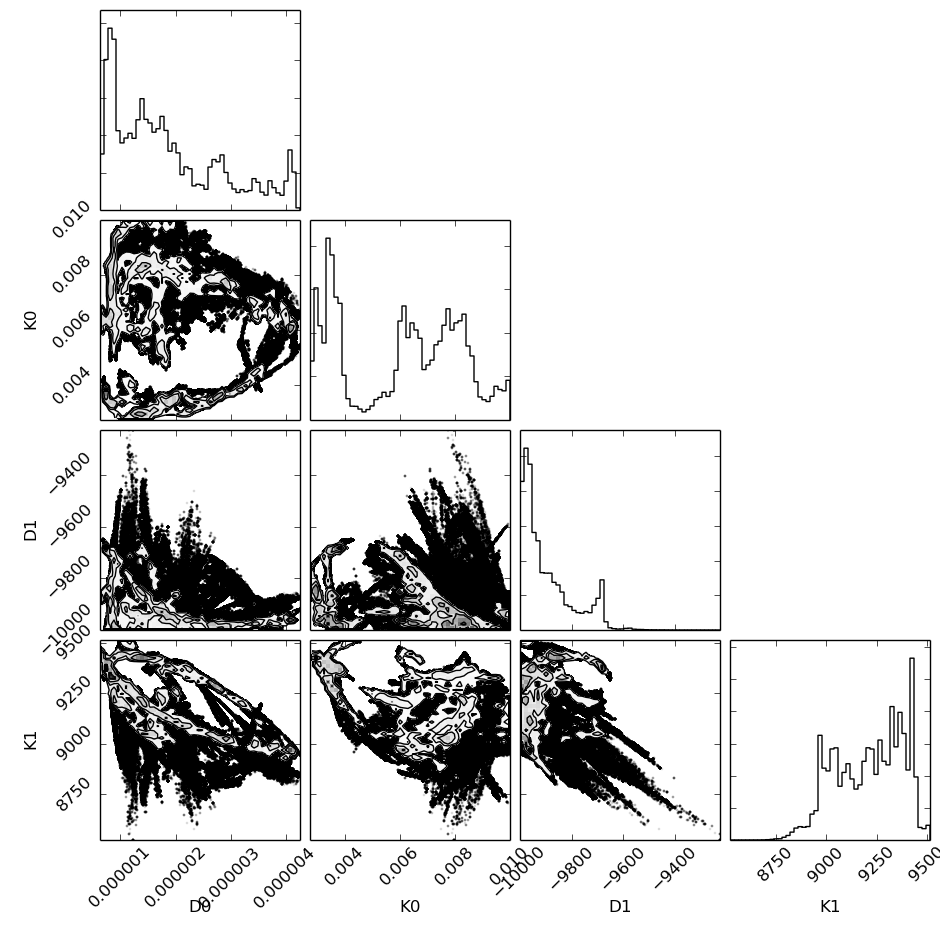
\includegraphics[width=0.48\columnwidth]{figs/1M_annealing_no_norm/triangle_seq_prior_3.png}
\\
n = 2 & n=3 \\
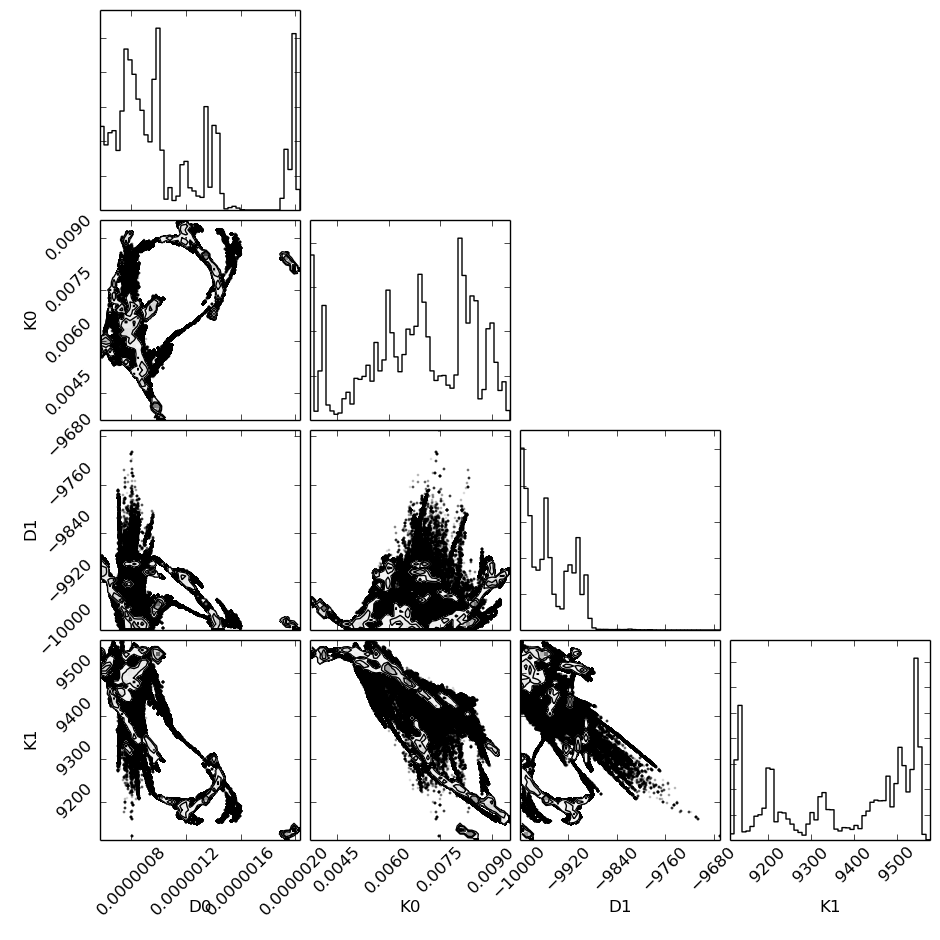
\includegraphics[width=0.48\columnwidth]{figs/1M_annealing_no_norm/triangle_seq_prior_4.png} \\
%& 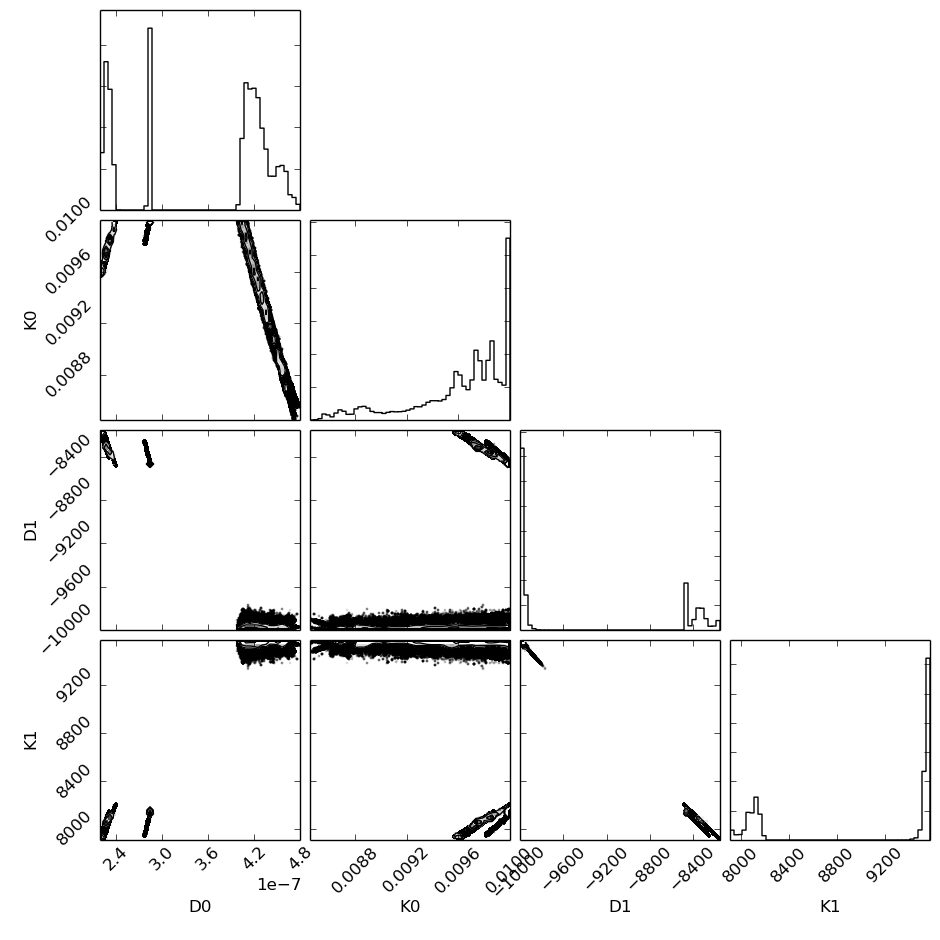
\includegraphics[width=0.48\columnwidth]{figs/1M_annealing_no_norm/triangle_seq_prior_5.png} \\
n = 4 & n=5 \\
\end{array}$
  \caption{Starting walkers uniformly across bounds, using
    annealing process where $\sigma = \sigma_0*(1+98)e^{-(5/4) n}$,
    where $n$ is the index of the pseudo-experiment. $n=4$ was
    experiment \#1 with $\sigma=\sigma_0$, and $n=5$ was both
experiments \#1 and \#2. $10^6$ samples per walker, no $1/N_m$ factor.}
  \label{fig:annealing_nonorm}
  \setfloatalignment{b}
\end{figure}

This time, the approach latches on to the `wrong' part of the distribution. 
It would seem that choosing 8 samples from the prior does not, unsurprisingly,
represent the prior in a meaningful way. 

%\newthought{To try to get around this I tried clustering the samples}
%using kmeans on the posterior samples (with $N_{walkers}+2$
%clusters)\footnote{Experimented with this a bit---using lots of
%  clusters, keeping best $N/2$ with small perturbations, etc}. Then I sorted these by the
%likelihood at the cluster centroid and kept the most likely $N$.
%Still didn't work well (see Figure~\ref{fig:annealing_clustering}).
%\begin{figure}
%$\begin{array}{c c}
%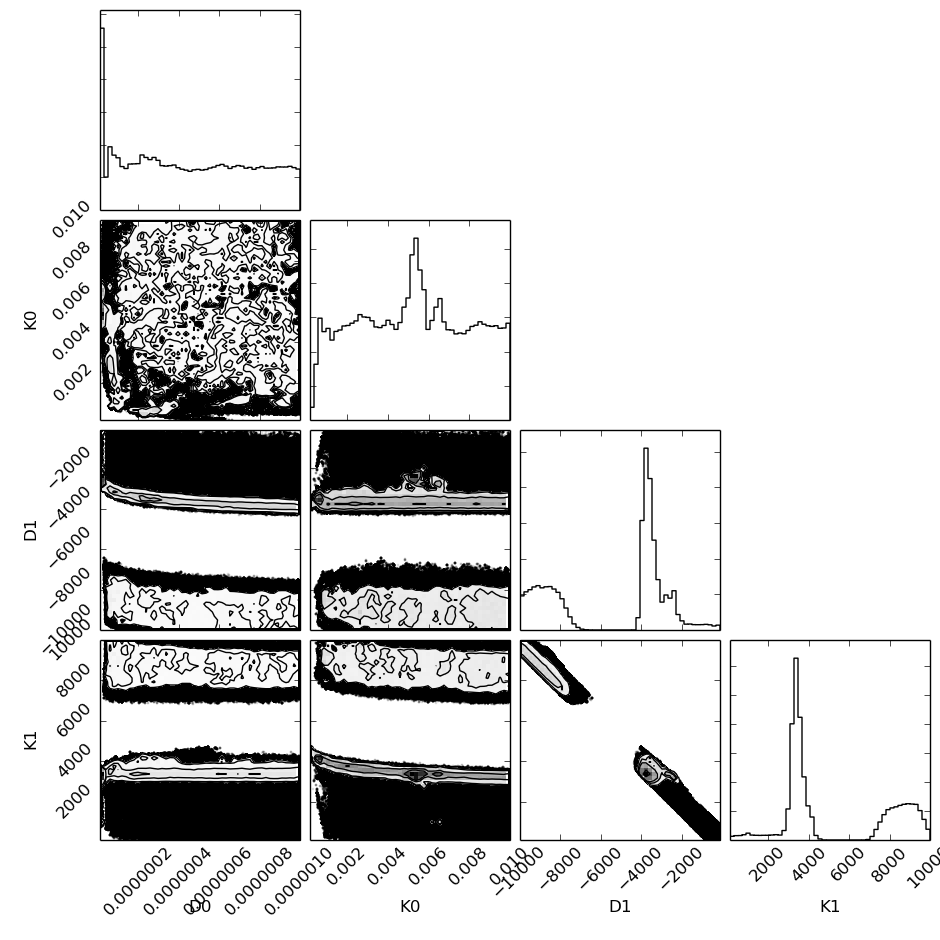
\includegraphics[width=0.48\columnwidth]{figs/long_annealing_clustering/triangle_seq_prior_0.png}
%& 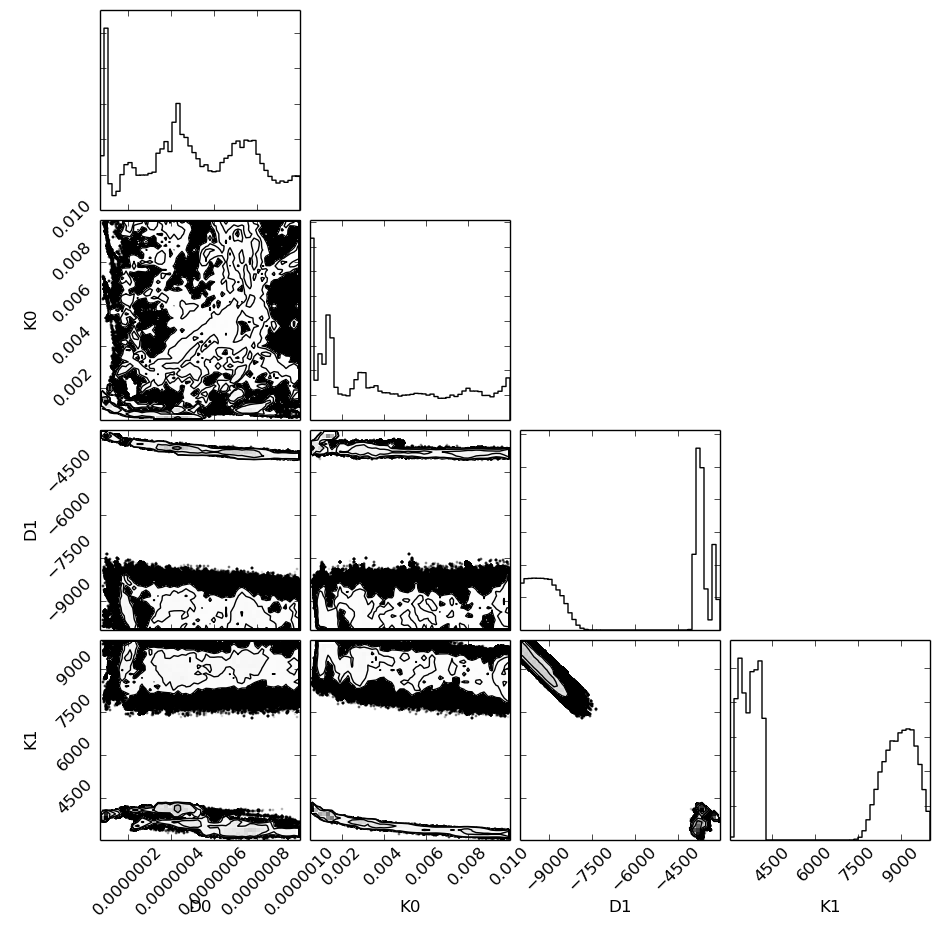
\includegraphics[width=0.48\columnwidth]{figs/long_annealing_clustering/triangle_seq_prior_1.png}
%\\
%n=0 & n=1 \\
%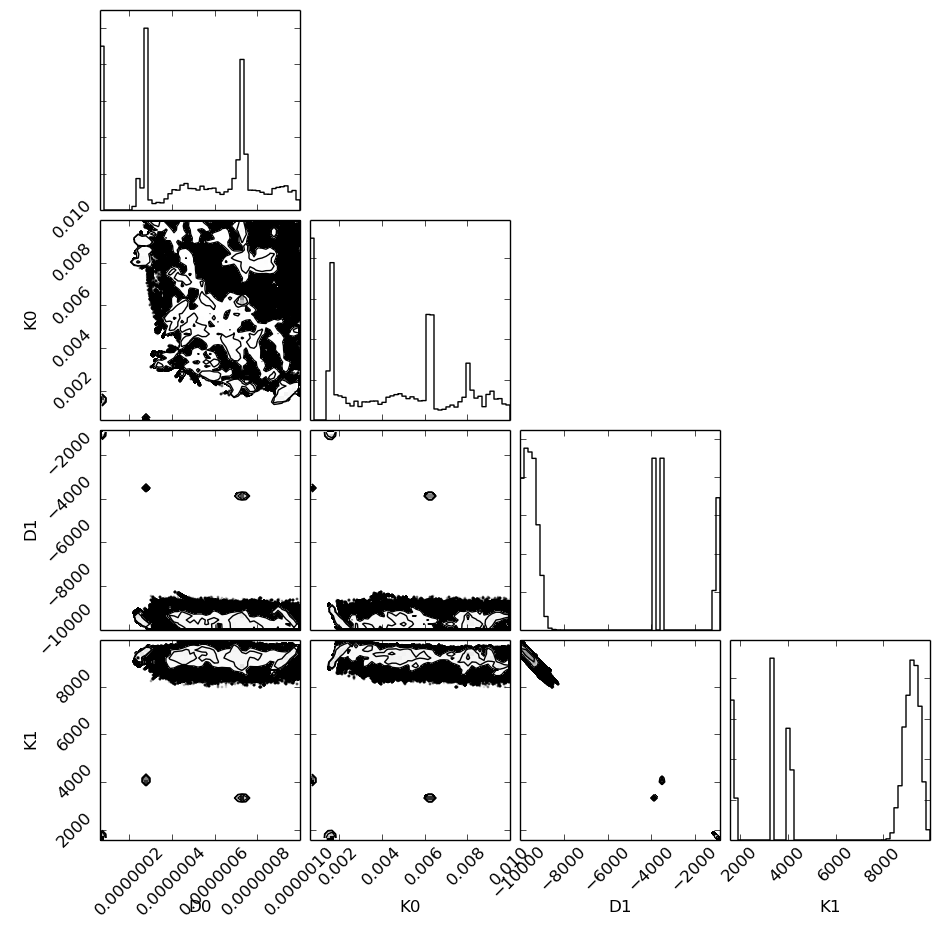
\includegraphics[width=0.48\columnwidth]{figs/long_annealing_clustering/triangle_seq_prior_2.png}
%& 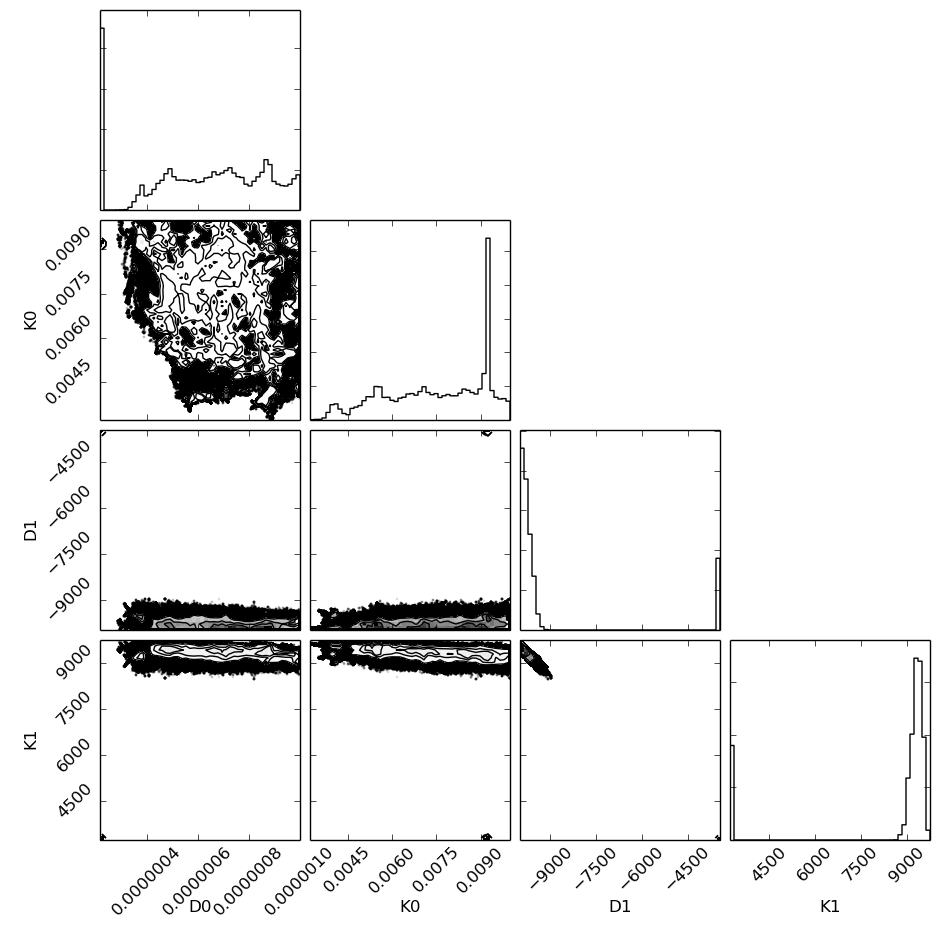
\includegraphics[width=0.48\columnwidth]{figs/long_annealing_clustering/triangle_seq_prior_3.png}
%\\
%n = 2 & n=3 \\
%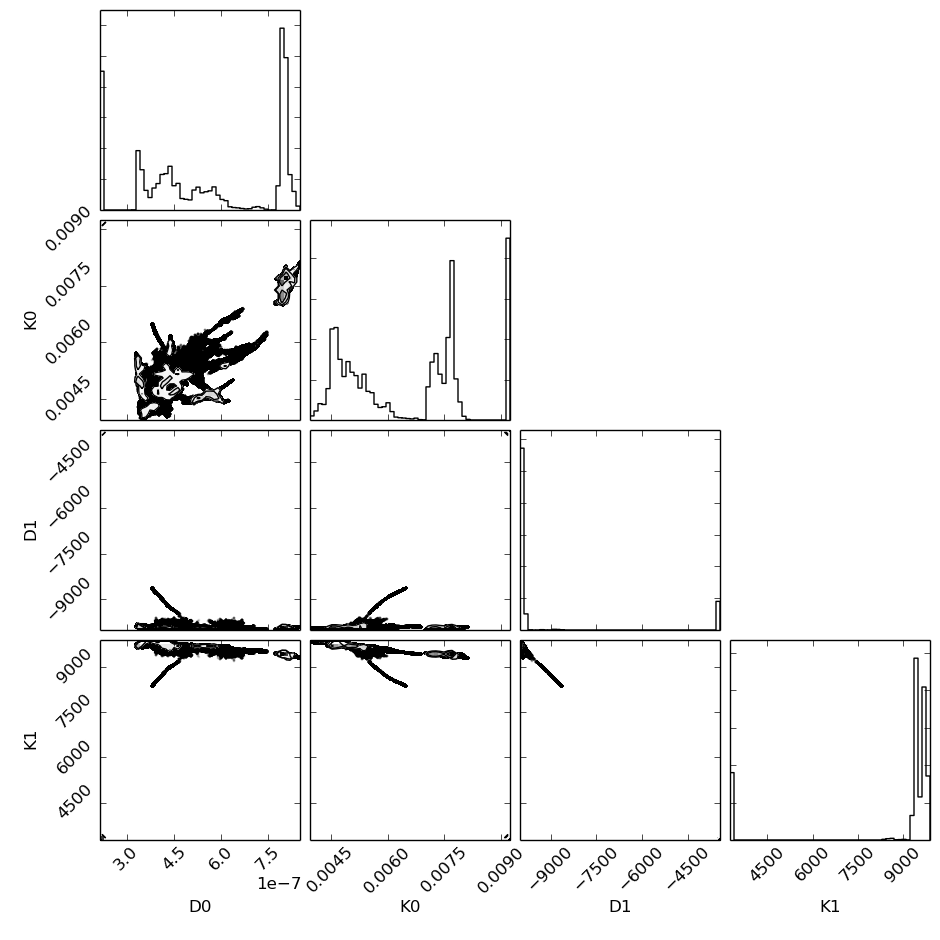
\includegraphics[width=0.48\columnwidth]{figs/long_annealing_clustering/triangle_seq_prior_4.png}
%& 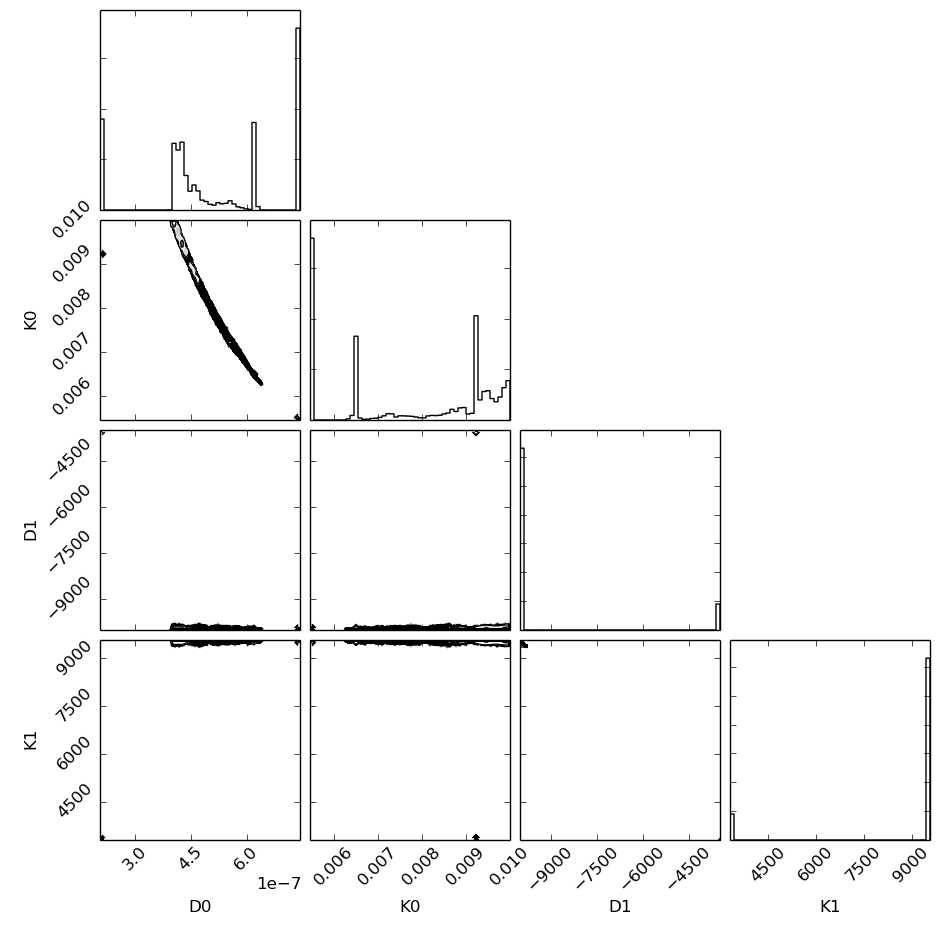
\includegraphics[width=0.48\columnwidth]{figs/long_annealing_clustering/triangle_seq_prior_5.png} \\
%n = 4 & n=5 \\
%\end{array}$
%  \caption{Starting walkers uniformly across bounds, using
%    annealing process where $\sigma = \sigma_0*(1+98)e^{-(5/4) n}$,
%    where $n$ is the index of the pseudo-experiment. $n=4$ was
%    experiment \#1 with $\sigma=\sigma_0$, and $n=5$ was both
%    experiments \#1 and \#2. $10^6$ samples per walker. Walker
%    positions based on clustering of previous samples.}
%  \label{fig:annealing_clustering}
%  \setfloatalignment{b}
%\end{figure}



\section{Sparse pdf}
Testing to see if it is sensible\ldots Test is:
\begin{itemize}
    \item Draw $10^6$ samples from normal distribution, use this to build sparse pdf representation $\mu_H$
    \item Draw $10^6$ samples from uniform distribution
    \item Reweight by probability from $\mu_H$
    \item Normalize weights so $\sum w_i = 1.0$
    \item Resample using Matti's routine
    \item Make triangle plots of both input and output distributions
\end{itemize}

\begin{figure}
$\begin{array}{c c}
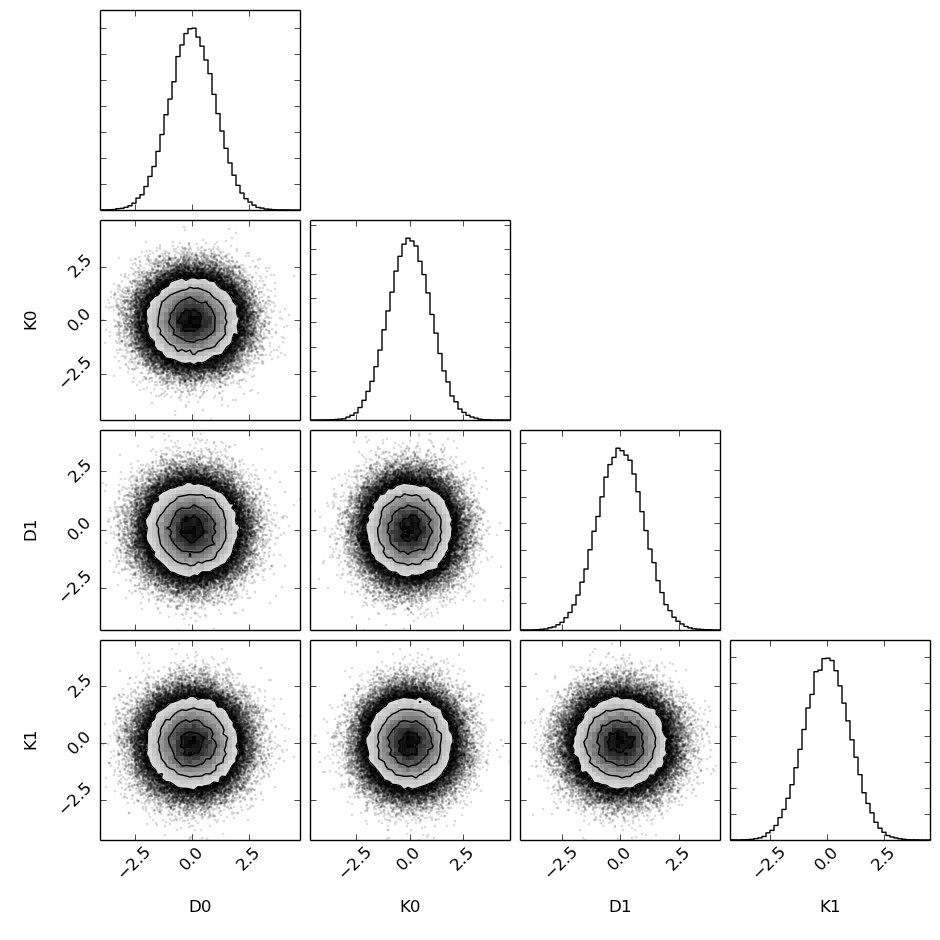
\includegraphics[width=0.4\columnwidth]{figs/input_samples.png}
& 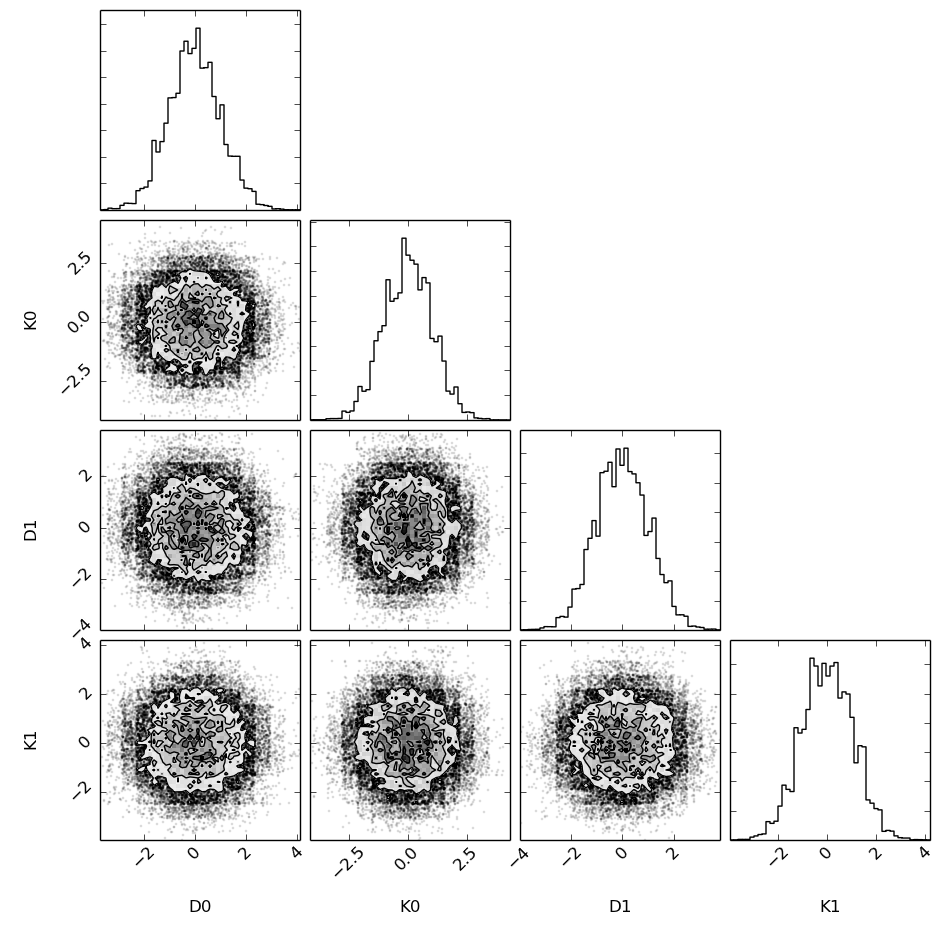
\includegraphics[width=0.4\columnwidth]{figs/spdf_samples.png}\\
\text{Input samples}& \text{Uniform samples weighted by $\mu_H$} \\
\end{array}$
\caption{If everything is working properly, these would be the same---the left
from the input samples, the right from what comes out of the histogram based
sparse pdf representation}
  \label{fig:spdf}
  \setfloatalignment{b}
\end{figure}

Although this is `working' as spec'd, it doesn't yet seem sufficient. When the
sample space isn't well filled out, the representation is pretty choppy.
Figure~\ref{fig:spdf_annealing2}, below, repeats the test in
Figure~\ref{fig:spdf} with some of the distributions from
Figure~\ref{fig:annealing2}. It seems like we need a better interpolation
routine.\footnote{I don't think RBF is it though, because as I understand it
    with RBF there is enough freedom that the interpolating function goes
    through every point. Here it seems like we want lower order interpolant
that enforces some smoothness, or to add TR style smoothing. }
\begin{figure}
$\begin{array}{c c}
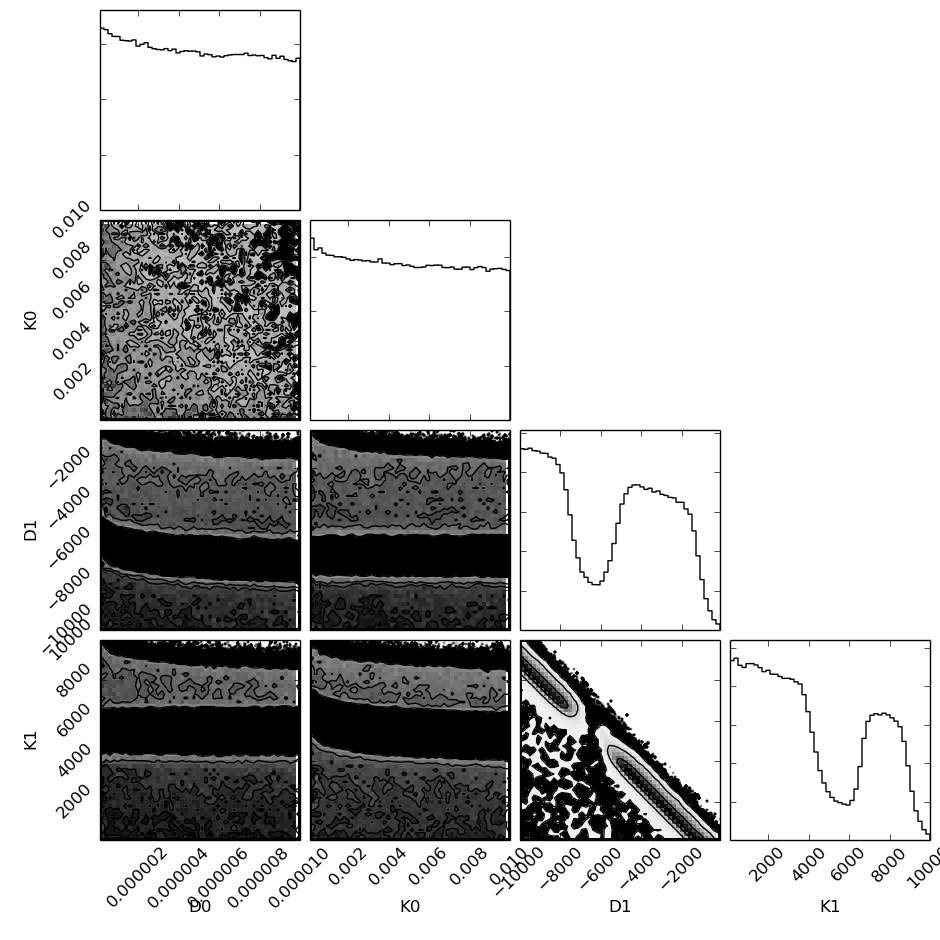
\includegraphics[width=0.48\columnwidth]{figs/1M_annealing_norm/triangle_seq_prior_0.png}
& 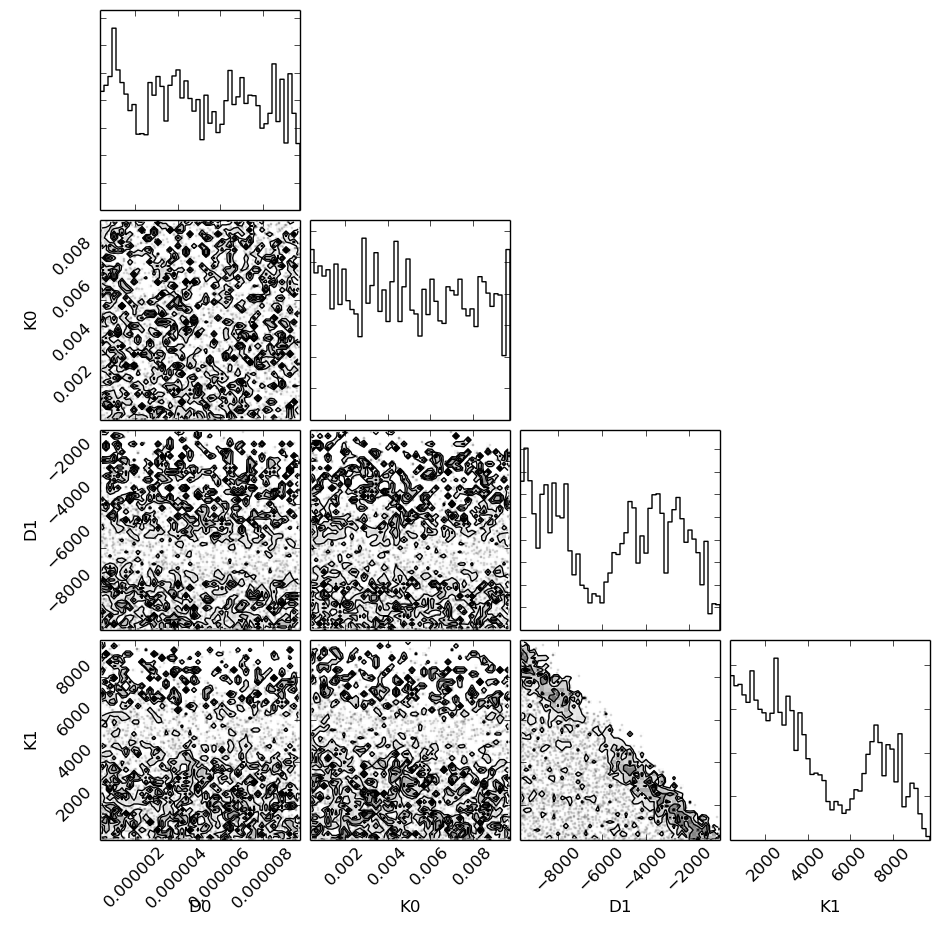
\includegraphics[width=0.48\columnwidth]{figs/1M_annealing_norm/triangle_seq_prior_spdf_0.png}
\\
n=0 & n=0 \\
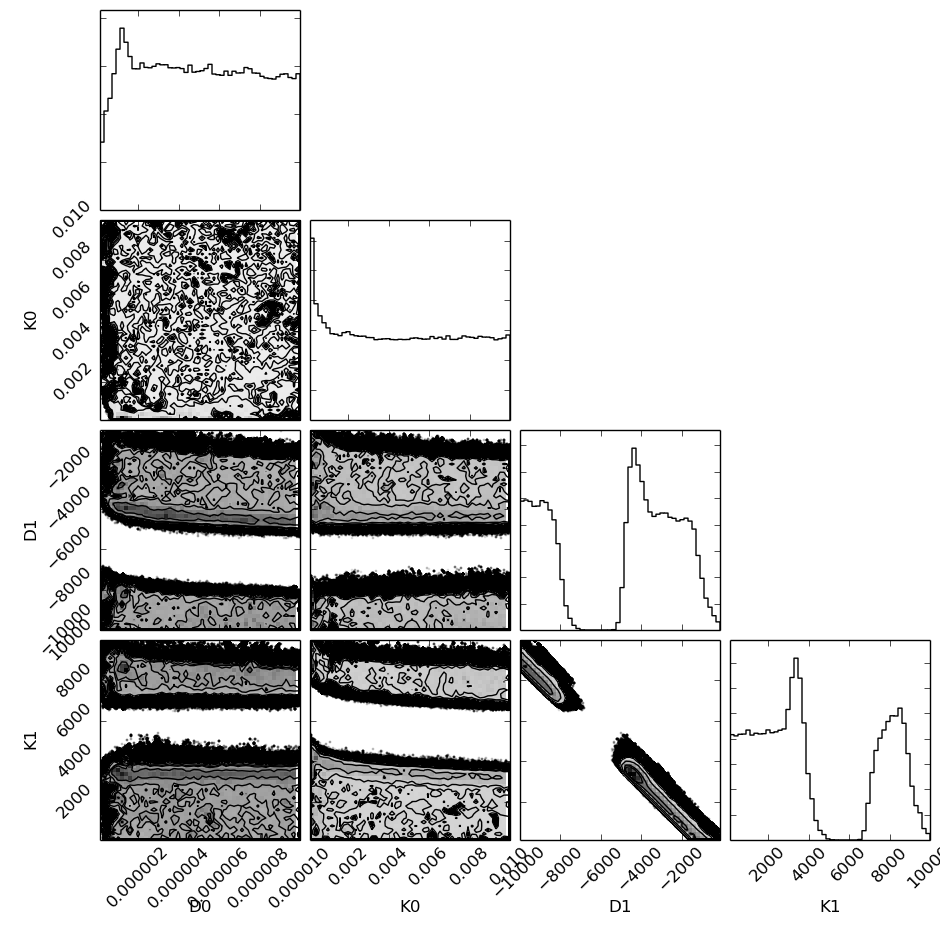
\includegraphics[width=0.48\columnwidth]{figs/1M_annealing_norm/triangle_seq_prior_1.png}
& 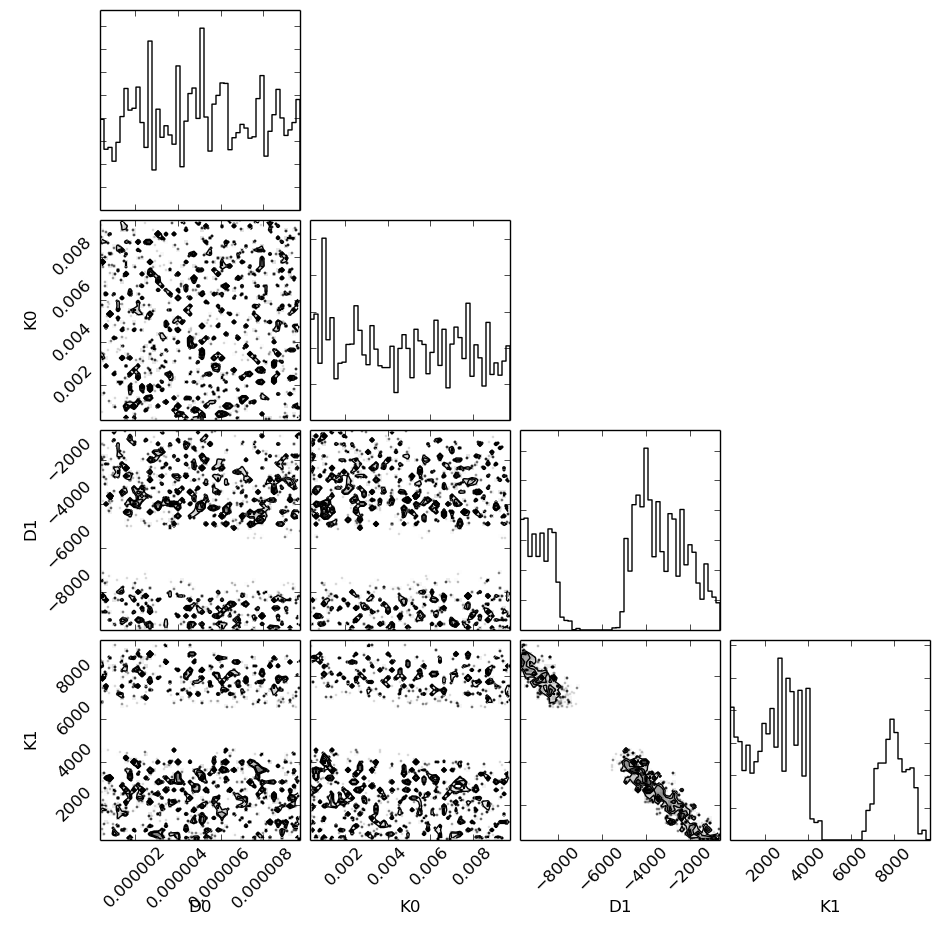
\includegraphics[width=0.48\columnwidth]{figs/1M_annealing_norm/triangle_seq_prior_spdf_1.png}
\\
n = 1 & n=1 \\
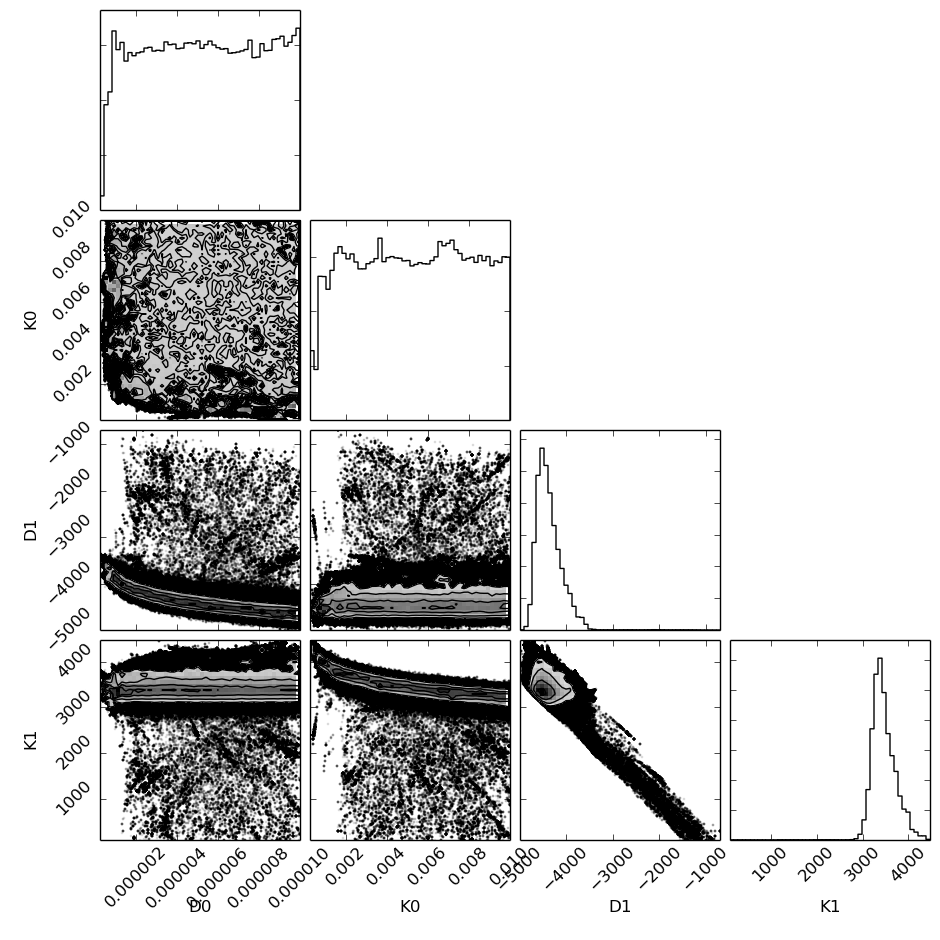
\includegraphics[width=0.48\columnwidth]{figs/1M_annealing_norm/triangle_seq_prior_2.png}
& 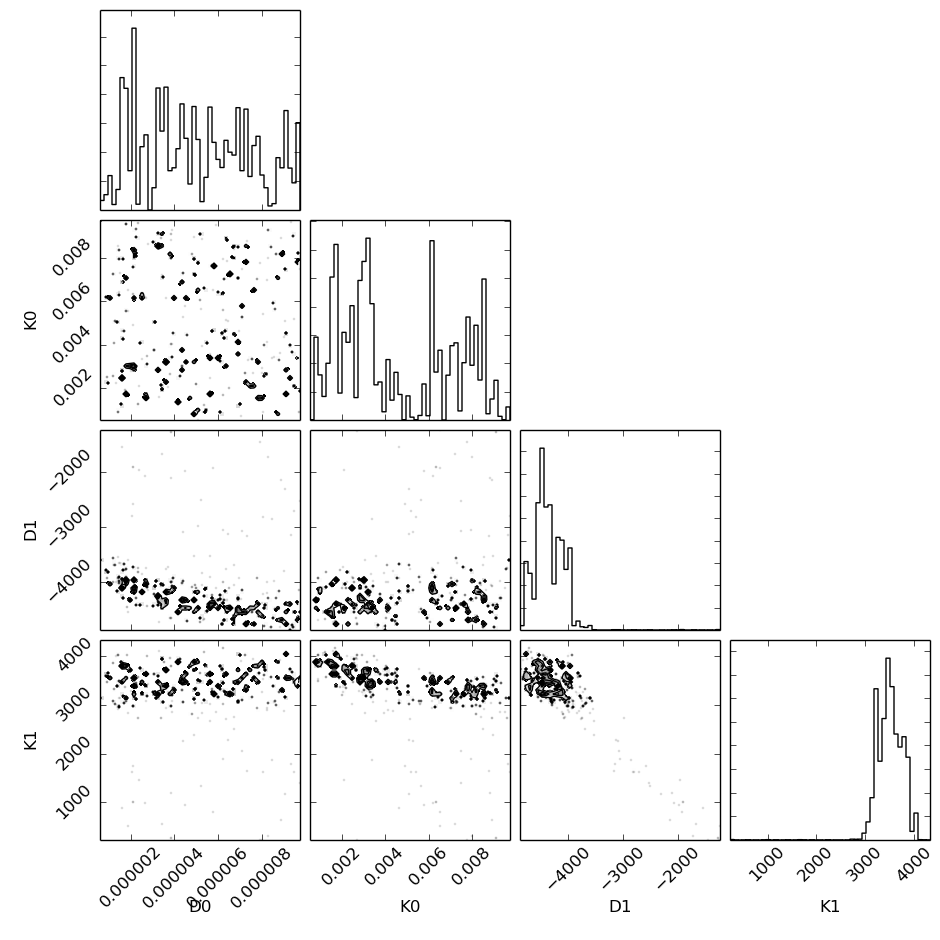
\includegraphics[width=0.48\columnwidth]{figs/1M_annealing_norm/triangle_seq_prior_spdf_2.png} \\
n = 2 & n=2 \\
\end{array}$
  \caption{Comparison of distributions from sampling and those recovered from histogram based weighting.}
  \label{fig:spdf_annealing2}
  \setfloatalignment{b}
\end{figure}
\clearpage
\section{Matti's notes on reweighting}
Assume we start with $M$ samples drawn from $p(\theta|z_2)$, either
from the emcee sampler or elsewhere. Then consider experiment \#1:
\begin{align}
  \label{eq:1}
  w & \propto \frac{ p(\theta|Z_1,Z_2) }{\pi(\theta; Z_1, Z_2)}\\
  & \propto \frac{ p(Z_1|\theta) p (\theta|Z_2)}{\pi(\theta; Z_1, Z_2)}
\end{align}

Choose $\pi(\theta; Z_1, Z_2) = p(\theta|Z_2)$, then
\begin{equation*}
  w \propto p(Z_1 | \theta),
\end{equation*}
which can be found simply by evaluating experiment \#1. 

An alternative view is, again starting with $p(\theta|Z_2)$,
\begin{align*}
  p(\theta|Z_1,Z_2) &= p (Z_1, Z_2 | \theta) \frac{
    p(\theta)}{p(Z_1,Z_2)} \\
& = \frac{p(Z_1|\theta, Z_2) p(Z_2|\theta) p(\theta)}{ p(Z_1,Z_2)}\\
 & = \frac{p(Z_1|\theta, Z_2)}{p(Z_1|Z_2)} \underbrace{\frac{p(Z_2|\theta)p(\theta)}{p(Z_2)}}_{p(\theta|Z_2)}
\end{align*}

\begin{align*}
  p(\theta|Z_1,Z_2)& \propto p(Z_1|\theta, Z_2) p(\theta|Z_2) \\
  & \approx p(Z_1|\theta) p(\theta|Z_2)
\end{align*}

Once the weights are determined, the initial $M$ samples can be
reweighted by the probability given the other experiments and resampled:
\begin{equation*}
  w(u_m) = \mathrm{lnlike}(u_m; Z_2)
\end{equation*}

Normalize, exponentiate:
\begin{equation*}
  w = w - \max(w)
\end{equation*}

\begin{equation*}
  w = e^w
\end{equation*}

\begin{equation*}
  w = \frac{w}{\sum w}
\end{equation*}
\begin{equation*}
  R = \mathrm{compR}(w)
\end{equation*}
\begin{equation*}
  N_{\mathrm{eff}} = M/R
\end{equation*}
\begin{equation*}
  X_{rs} = \mathrm{resampling}(X,w) \sim p(\theta|Z_1,Z_2)
\end{equation*}

\section{Next plan}
\begin{enumerate}
    \item Solve for MLE for Expt. \#1 (by itself), and evaluate Hessian\footnote{
        This I don't think is a good idea, because it introduces the
            complicating matter of degeneracy. I will try in a bit using \#1
        and \#2 together, then adding \#3.}
\item Use the inverse of the Hessian as covariance for the 'prior',
  draw the initial walker positions from this\footnote{Maybe still use a
    `broad prior', but use this instead of \emph{ensemble\_std}}
\item Run the hammer
\item Use the covariance of the samples as the covariance for a new ball
  of walkers (N-d normal) for sampling Expt. \#1 and \#2 together.\footnote{Where
    to center the ball? At the most likely of the samples evaluated?}
\item Also try impilcit sampling on this
\end{enumerate}

\section{Progress on implicit sampling}
\newthought{Going ahead with trying to evaluate the Hessian} using the first
two experiments by finite difference produces a reasonable result, with
eigenvalues all of the same sign. I may not have done this quite right, but it looks reasonable to me. What I did was:
\begin{enumerate}
    \item Solve for MLE of parameters; evaluate Hessian using finite difference about this point
    \item Find inverse of Hessian using numpy.linalg.inv
    \item Find eigenvalues using numpuy.linalg.eigh(Hinv) and check that they all had same sign. 
    \item Draw 50k samples from a multivariante normal using numpy.random.multivariate\_normal with mean from MLE estimate and cov=Hinv. 
    \item For each sample:
        \begin{itemize}
           \item evaluate $F0$ using scipy.stats.multivariate\_normal.pdf with mean from MLE and cov=Hinv
           \item For each sample also evaluate $F1$ using data from Exp. \#1 and \#2.
           \item $w_i = -F0 + F1$
       \end{itemize}
   \item Then rescale weights: $w_i = exp(w_i - w_{max})$
   \item Then normalize weights: $w_i = w_i/\sum(w_i)$
    \item Finally, use Matti's resampling routine to get new samples
\end{enumerate}
The outcome of all this is shown in Figure~\ref{fig:is}
\begin{figure}
$\begin{array}{c c}
    \includegraphics[width=0.48\columnwidth]{figs/is_test/no_norm/triangle_Hinv.png}
    & \includegraphics[width=0.48\columnwidth]{figs/is_test/no_norm/triangle_RS.png}\\
    \text{Input samples} & \text{Resampled samples} \\
\end{array}$
\caption{Implicit sampling result for combination of Experiments \#1 and \#2, no $1/N_m$ factor.}
  \label{fig:is}
  \setfloatalignment{b}
\end{figure}

\begin{figure}
$\begin{array}{c c}
    \includegraphics[width=0.48\columnwidth]{figs/is_test/norm/triangle_Hinv.png}
    & \includegraphics[width=0.48\columnwidth]{figs/is_test/norm/triangle_RS.png}\\
    \text{Input samples} & \text{Resampled samples} \\
\end{array}$
\caption{Implicit sampling result for combination of Experiments \#1 and \#2, with $1/N_m$ factor.}
  \label{fig:is}
  \setfloatalignment{b}
\end{figure}

\section{More progress}
\bibliographystyle{plainnat}



\end{document}

